%!TEX root = ../../dissertation.tex
%%%%%%%%%%%%%%%%%%%%%%%%%%%%%%%%%%%%%%%%%%%%%%%%%%%%%%%%%%%%%%%%%%%%%%%%%%%%%%%%
\chapter{Evaluating Reliable Streaming in Mobile Networks}
\label{chap:mobilestreaming-measurements}

Testing and evaluation plays a crucial role not just in correctly utilizing cross-layer data but also for media streaming in mobile networks in general. All of the discussed layer influences, interactions and other unintentional side-effects need to be thoroughly understood for the intended goal of optimizing reliable streaming in mobile networks.

The core network trace evaluations undertaken in Chapters~\ref{chap:mobilenets} and \ref{chap:mobilenetsmeasuring} were already able to highlight the load influencing dynamics of the core network control plane. But many more aspects remain uninvestigated, some of which may not even be covered by this kind of passive network-wide measurement type.

To further the understanding of the behavior of reliable streaming in mobile networks and investigate influence sources, usually either active measurements or simulations are conducted. Both methods and their drawbacks and benefits are discussed in this chapter. Moreover, an approach to enhance active measurements for mobile devices, that facilitates meta-data of the device and improve measurement accuracy, is presented in the first section. Afterwards, a full \gls{LTE}-based reliable streaming simulation is also introduced and some initial results are given.



%%%%%%%%%%%%%%%%%%%%%%%%%%%%%%%%%%%%%%%%%%%%%%%%%%%%%%%%%%%%%%%%%%%%%%%%%%%%%%%%
%!TEX root = ../../dissertation.tex
%%%%%%%%%%%%%%%%%%%%%%%%%%%%%%%%%%%%%%%%%%%%%%%%%%%%%%%%%%%%%%%%%%%%%%%%%%%%%%%%
\section{Active Measurements and Testbeds}
\label{c6:sec:active-measurements}

Active measurements includes any kind of approach that generates its own network traffic and bases the evaluation on it. Therefore, they are usually conducted on an end-to-end base, with at lest one side under the control of the experimenter.

Apart from researchers writing their own specialized application for a singular study, active measurements are most often conducted with the help of existing network testbeds, thereby reducing the overall effort.
Any new or an alteration to existing network protocols are usually best tested in large-scale network testbeds to collect performance data and find side-effects. The presence of background traffic and a large device heterogeneity and diversity are often considered an advantage to a testbed as it better resembles real networks.

Testbeds can be either physically constructed by setting up a number of dedicated machines in a lab or form a virtual overlay spanning over an existing computer network. Both of these principles work well for wired network and there are a lot of examples of successful testbeds constructed with these principles.

Currently one of the largest installations is PlanetLab~\cite{chun2003planetlab}, consisting of dedicated machines located at a number of University sites. An experimenter can instantiate a \textit{slice} --- a portion of the overlay network made up of number of interconnected \glspl{VM} hosted on the various machines --- and conduct her studies. Thus, many experiments can run concurrently.

Several testbeds devote themselves to wireless and mobile networks. These are usually either put together in a clean lab environment, SmartLab\footnote{\url{http://smartlab.cs.ucy.ac.cy/}} or 
EmuLab\footnote{\url{http://www.emulab.net/}} come to mind, or hand out subsidized mobile devices prepared with custom firmwares to volunteers which need to allow running network experiments on them. The approach is taken, e.g., by NetSense~\cite{Striegel:2013:LLN:2491159.2491171} and PhoneLab\footnote{\url{https://www.phone-lab.org/}}~\cite{Nandugudi:2013:PLP:2536714.2536718}. The latter approach raises some interesting issues concerning the volunteers' privacy which will be covered in the next section.

All of these testbeds consist of rather uniform nodes and access to it still requires some amount of administrative effort, alternative approaches are also available, for example in the form of the Seattle Testbed\footnote{\url{https://seattle.poly.edu/html/}}~\cite{Cappos:2009:SPE:1508865.1508905}. Its overlay network comprises of small software sandboxes installable on a wide range of device types. Experimenters gain automatic access to a portion of the overlay through a clearing house and are resource-restricted to their slice by a hypervisor. As Seattle is available to both conventional desktop and server computers as well as Android smartphones, the overlay composition very heterogeneous. Therefore, the node stability and availability can vary substantially over time, caused amongst other things by the individual uptime of the computers following typical diurnal cycles and mobility-related connectivity issues.
While this forms a much more realistic picture of a network, it simultaneously makes the execution of the actual study more difficult as these churning issues have to be dealt with.

The requirements for conducting reliable streaming experiments are low. As it is usually a fully pull-based approach, full control over the server containing the streaming files is not necessary. It is also generally not necessary to display the actual video on the client in reliable streaming as it always will be a pixel-perfect representation. Therefore, the buffer-emulation measurement approach presented in \ref{c3:sec:measurements} can be employed here. The measurement devices only have to record the transmission traces of the streaming process and make them available to the emulation process. The latter can for example also be performed in a centralized and asynchronous matter when dealing with non-adaptive streaming.


%%%%%%%%%%%%%%%%%%%%%%%%%%%%%%%%%%%%%%%%%%%%%%%%%%%%%%%%%%%%%%%%%%%%%%%%%%%%%%%%
\subsection{Enriching Mobile Measurements with Additional Metadata}
\label{c6:sec:sensorium}

While transmission traces might be the bare minimum to conduct reliable streaming measurements, meaningful mobile measurement can include much more metadata, giving insightful indication of the device's current state.

Mobile devices have access to a vast array of data. On the one hand does the networking stack itself much information on its state, as discussed in the previous Chapter. The current radio and mobility state is especially relevant to mobile streaming measurements as it directly influences the link's \gls{QoS} parameters. 

But modern mobile devices additionally contain an ever-growing number of sensors, including \gls{GPS}, accelerometers, temperature, pressure, luminosity, humidity, fingerprint, heartbeat, and several cameras and microphones. Moreover, further radio interfaces (WiFi, Bluetooth, \acrshort{NFC}) gather data on network availability and signal quality. Each additional data source can help in quantifying the physical position, orientation and state of the device and even quantify the ``state'' of its user. Even the NSA is allegedly more interested in metadata in general than actual data for this reason.\footnote{\url{http://www.wired.com/2013/06/phew-it-was-just-metadata-not-think-again/}}

Active measurements in mobile networks should make use of metadata and correlate it to the regular measurement data to achieve a finer result granularity. Alternatively, sensor data can also be used for new kinds of evaluations. Questions like ``Can this device watch video at a an satisfactory quality at certain locations?'' can be raised and answered.


%%
\subsubsection{Metadata and Privacy}

While the actual experiment usually runs in a strict sandbox environment with no access to actual data on the device, allowing sensor and metadata access creates holes in the isolation model. As informative metadata can be for network studies as intrusive is unmediated access to this data for the device's user.

In a pure lab environment this poses no problem as there will be no device owner whose information can be leaked. However, preserving the privacy of actual device users running network testbed software is absolutely critical for a number of reasons:

\begin{itemize}

	\item For ethical reasons as stated in several ethics proclamations, for example in the well-known hacker ethics\footnote{\url{http://www.ccc.de/hackerethics}} which states to \textit{``Use public data, protect private data.''}. This is often called the principle of data economy and minimalization, aiming to prevent abuse and minimize the effects of accidental data leakage.

	\item User acceptance is a very important aspect. Testbeds need to have a sufficiently large installation base to achieve meaningful results. But users might choose not to participate if the testbed application is too intrusive. There needs to be a balance between revealing and protecting privacy sensitive data. The acceptance can also be increased by information and disclosing employed data. This servers the additional purpose of educating the user of privacy sensitive data.

	\item Lastly, there are legal constraints to consider when dealing with personal information. In Germany, for example, several fundamental constitutional rights restrict the use of personal data. These are the \textit{``Recht auf informationelle Selbstbestimmung''}\footnote{\url{https://www.bmi.bund.de/DE/Themen/Gesellschaft-Verfassung/Datenschutz/Informationelle-Selbstbestimmung/informationelle-selbstbestimmung_node.html}} and the \textit{``Grundrecht auf Gewährleistung der Vertraulichkeit und Integrität informationstechnischer Systeme''}\footnote{\url{https://www.bundesverfassungsgericht.de/entscheidungen/rs20080227_1bvr037007.html}}.

\end{itemize}

To conclude, network measurement testbeds have to regulate, filter, adjust, or outright prevent access to sensitive data. Existing testbeds usually do not take a technical but rather a bureaucratic approach to this problem. For example, all experiments in the aforementioned PhoneLab require approval from a review board.

But that does not mean, that there are no technical means available. Looking outside of the field of network testbeds, some research and even usable implementations are available.

A very basic and static approach to protecting privacy data is implemented in the regular versions of both iOS and Android. On installation any application has to request specific rights for each sensor source to be able to use it in the future. 
The ``Privacy Guard'' feature\footnote{\url{https://plus.google.com/+CyanogenMod/posts/gk7X3HjNvnH}} in the custom Android firmware CyanogenMod\footnote{\url{http://cyanogenmod.org/}} provides the additional capability to monitor and revoke any sensor permissions at runtime.

Other approaches include increasing the permission granularity~\cite{Jeon:2012:DAM:2381934.2381938} or tagging sensor data at the source to better track and find privacy leaks in Applications~\cite{enck2010taintdroid}.


%%
\subsubsection{Preserving Testbed User Privacy with Sensorium}

Even with these approaches at hand, the privacy issue should be mitigated further beyond the binary allow/deny access approach. Also, it usually is a complicated task for experimenters to access all the various sensors,each answering to a different \gls{API}. \textit{Sensorium}~\cite{raf2013sensorium} was created to remedy both of these issues. Sensorium is a generic unified sensor reading framework that interfaces with other applications as well as network nodes and provides the sensor readout to them. More importantly, a fine-grained multi-level privacy control model is implemented.


%%
\paragraph{Architecture}

\begin{figure}[htb]
	\centering
	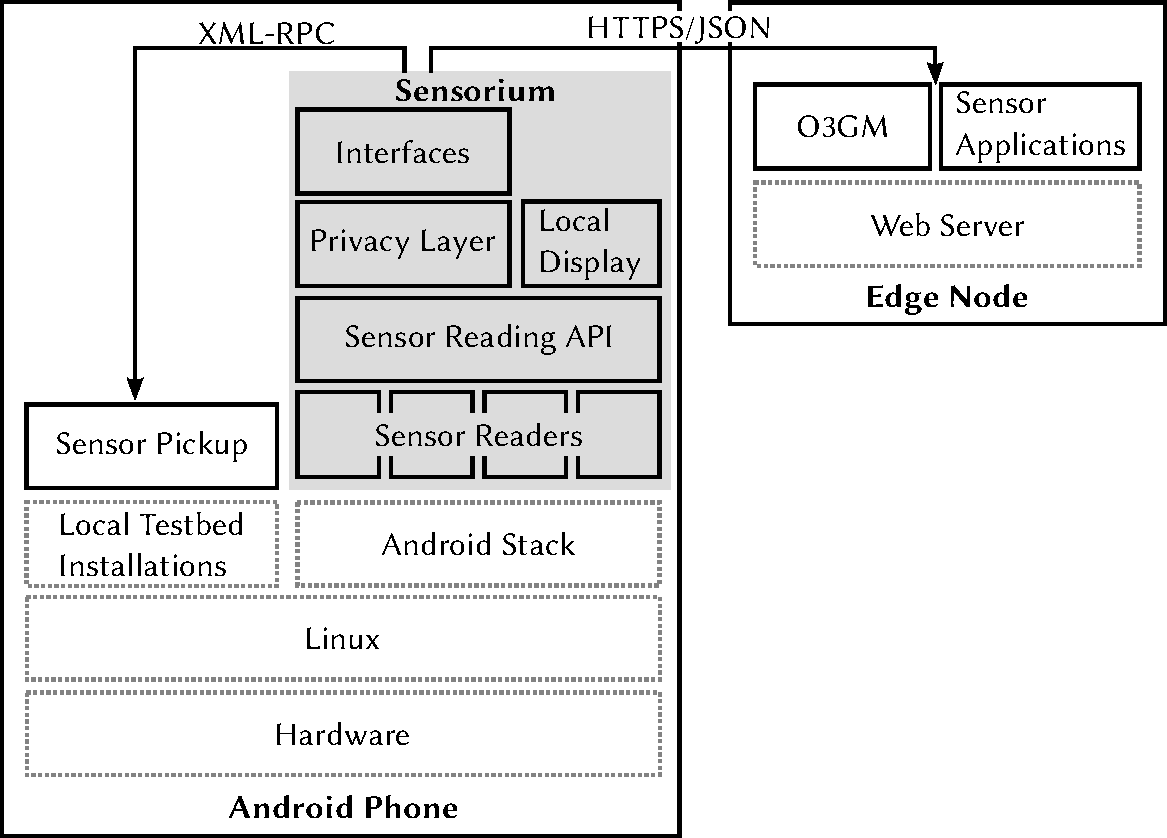
\includegraphics[width=0.8\textwidth]{images/sensorium-arch.pdf}
	\caption{Sensorium architecture interfacing with other applications. Previously existing components are marked with a dotted line.}
\label{c5:fig:architecture}
\end{figure}

Figure~\ref{c5:fig:architecture} overviews the components of Sensorium's architecture The individual \textit{sensor drivers} are placed on top of the operating system and take care of reading sensor values from platform-specific interfaces and pushing them upwards into a common registry to be read by the \textit{sensor reading \gls{API}}. All sensor data is relayed both to a local display as well as to all \textit{outbound interfaces}. Due to the layered architecture, contributors can simply extend or substitute the existing layers. For example, new drivers or outbound interfaces can be easily implemented. 

The outbound interfaces include an \gls{HTTPS} client, that pushes \acrshort{JSON} data to any active network experiment server where the data can be further processed. To connect to programs running locally on the same device, the \acrshort{XML}-\acrshort{RPC} interface can be polled. Pull-based access from sources other than the local host is not allowed for security reasons. However, any data leaving Sensorium must first pass through the \textit{privacy layer}, which filters the data based on the user's preferences.


%%
\paragraph{Privacy Model}

This privacy layer allows for a fine-grained control over the amount and precision of data that the system is sharing. A settings \gls{GUI} provides the user full control over his privacy. Here, she can choose the amount of information she is willing to reveal for each sensor. Based on this preference, the privacy layer then either outright prevents access to specific values or reduces their impact by anonymizing them.

This anonymization task can work in several levels. Apart from completely replacing it with a running number, the value could also be hashed. In many cases context-sensitive anonymization approaches are available. For example, the precision of a geo-location could simply be reduced down to a city-level or even country-level.

As the user is always in firm control of the process, she should be more accepting of actual network experiments that use this kind of data. However, such studies need also cope with the fact, that they might get incomplete or partially anonymized data.


%%
\paragraph{Implementation}

Sensorium is currently targeted at and implemented on the Android platform.\footnote{\url{https://github.com/fmetzger/android-sensorium}} It can be installed on any Android without any modification. Screenshots of the sensor display and settings menu of the application are depicted in \ref{c5:fig:sensorium}. Drivers for most of the typically available sensors are implemented.

\begin{figure}[htb]
	\centering
	\begin{subfigure}[b]{0.45\textwidth}
		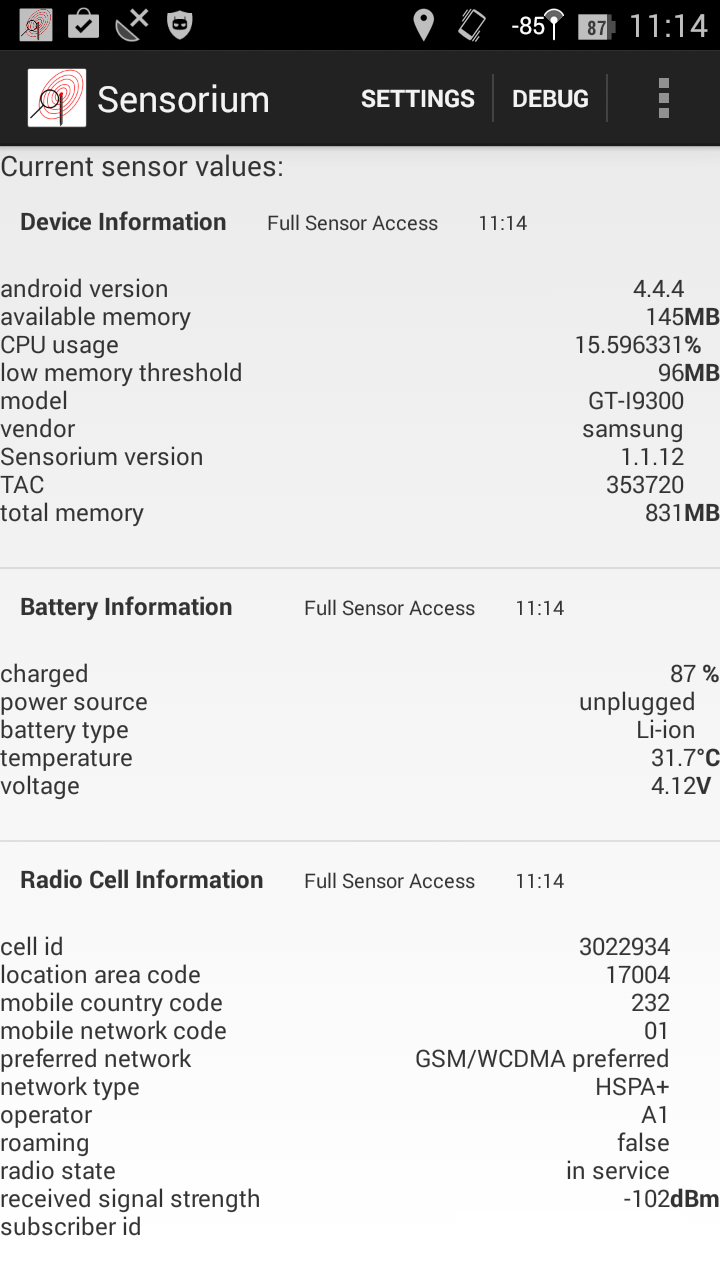
\includegraphics[width=\textwidth]{images/sensorium.png}
		%\caption{Stalling occurs without handover hinting.}
		%\label{c5:fig:streaming-hinting-no-cl}
	\end{subfigure}%
	\hfill
	\begin{subfigure}[b]{0.45\textwidth}
		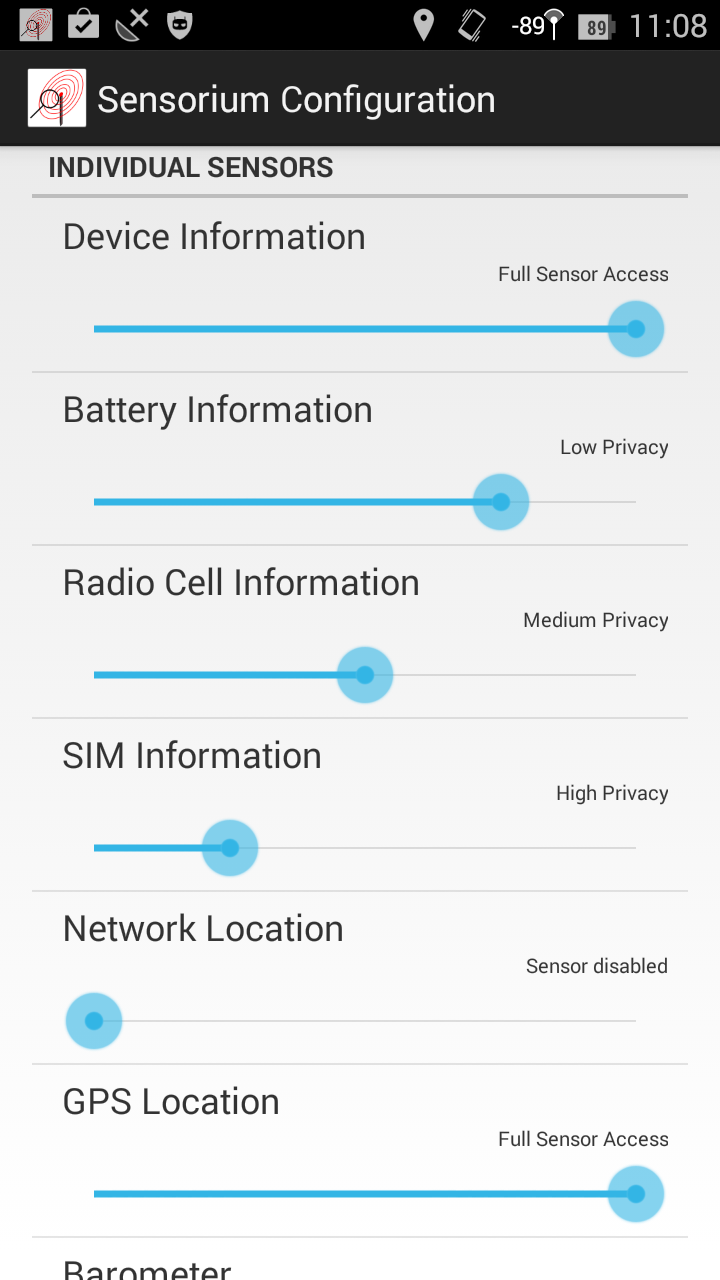
\includegraphics[width=\textwidth]{images/sensorium-settings.png}
		%\caption{Stalling can be prevented by hinting and proactively filling the playback buffer.}
		%\label{c5:fig:streaming-hinting-cl}
	\end{subfigure}%
	\caption{Sensorium sensor values display and settings screenshots.}
\label{c5:fig:sensorium}
\end{figure}

Sensorium was demoed at the NetSys 2013 conference and has since then been available in various app stores. Data from the Google Play Store suggests at least \numprint{50} concurrently running device installations across several countries, carriers and device types. Albeit a still low number, as there was no real advertisement conducted, this could indicate its feasibility as a companion application to a network testbed.

Of note are also two related applications, that intend to follow up on Sensorium's approach in the future: The Sensibility Testbed\footnote{\url{https://sensibilitytestbed.com/}}, which tightly couples itself to the aforementioned Seattle platform, and BlurSense\footnote{\url{https://blursense.poly.edu/}}~\cite{6798970}, aiming to improve the sensor value anonymization efforts. 


%%
\paragraph{Sensorium Usage}

Sensorium was originally written for two specific targets.

First, it was intended as a prototype sensor extension to the Seattle testbed. Pre-anonymized data was to be delivered through the \acrshort{XML}-\acrshort{RPC} interface to a locally running Seattle installation. Any experiment running in this sandbox could then facilitate this sensor data.

\begin{figure}[htb]
	\centering
	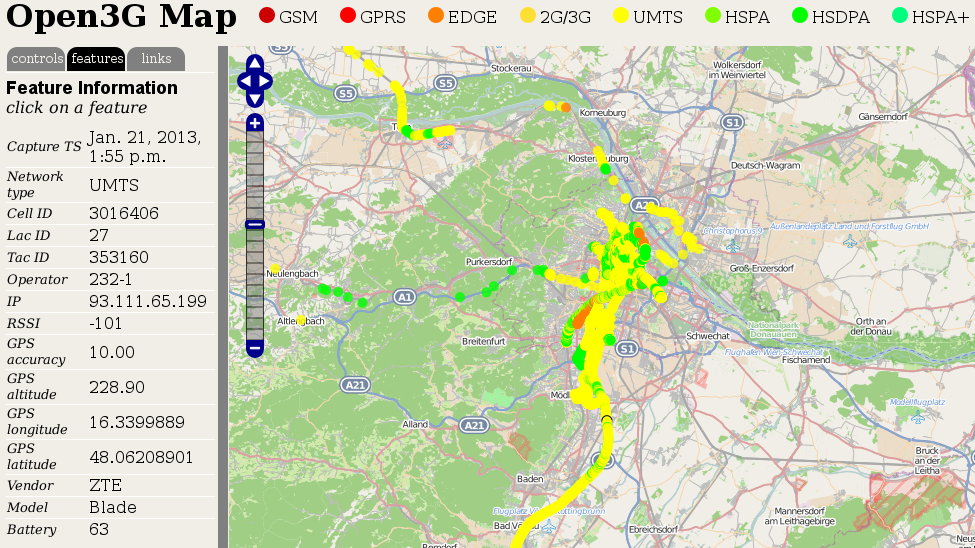
\includegraphics[width=\textwidth]{images/o3gm.png}
	\caption{The \gls{O3GM} web page, displaying a \gls{3G} coverage measurements layer with data collected by Sensorium on top of the OpenStreetMap base layer.}
\label{c5:fig:ogggm}
\end{figure}

Second, to present what actually can be done with smartphone sensing data, \gls{O3GM}\footnote{\url{https://o3gm.cs.univie.ac.at/o3gm/}}\footnote{\url{https://github.com/lukpueh/Open3GMap}} was created, which visualizes mobile coverage data. \gls{O3GM} is a Web service, that makes use of Sensorium's \acrshort{JSON} upload feature, displaying geo-located \gls{3G} radio access quality information in an OpenStreetMap overlay (using OpenLayers\footnote{\url{http://openlayers.org/}}) as can be seen in Figure~\ref{c5:fig:ogggm}

Coverage data is usually only available to mobile operators, which have not interest to share this information. Other projects such as OpenSignalMaps\footnote{\url{http://opensignal.com/}} and Sensorly\footnote{\url{http://www.sensorly.com/}}, as well as corporations like Google and Apple collect these data, but are very restrictive regarding usage by third parties. \gls{O3GM} data is freely available under an open content license.

Coverage data can again also be helpful to determine the viability of mobile reliable streaming. For example, knowing the \gls{RAT} and signal strength of a specific path can help make informed decisions on which stream quality to choose at which time for adaptive streaming.


%Improving wireless network performance using sensor hints \cite{ravindranath2011improving}


% HomeLab: A Platform For Conducting Experiments With Connected Devices In The Home \cite{Singh:2013:HPC:2486001.2491701}
% authentication-based privacy, fully up to the experimenter

% phonelab privacy approach:
% Large (288 devices) smartphone testbed
% each participant can choose to participate in individual experiments
% open for experimenters upon approval, centralized experiment execution by the review board
% privacy guaranteed only through the project review board, not through technical means (centralized, not distributed)
% bureaucratic apprach to experimentation and privacy, not automatized
% relies on Androids privacy mechanisms (imho: do not work for this type of project)
% real people (as opposed to emulab, planetlab,...)!
% interesting study for wifi->3g vertical handover locations -> could extend wifi coverage studies and wifi planning

%http://campar.in.tum.de/Chair/KalmanFilter
%https://dsp.stackexchange.com/questions/320/is-a-kalman-filter-suitable-to-filter-projected-points-positions-given-euler-an/321\#321
%``Sensor Fusion''?

%https://guardianproject.info/

% NativeWrap \url{http://research.csc.ncsu.edu/security/nativewrap} \cite{Nadkarni:2014:NAH:2627393.2627412}
% Use website as app instead of native app, thus reducing permissions


% Sensorium play store stats:
% usage peak: 51 concurrent device installs August 2014
% total installs: 475 as of august 2014
% on various types of devices (including tablets)
% across several countries (top: US, DE, AT, India, Turkey)
% and all carriers
% with not particular advertisement (demo presentation at one national conference NetSys 2013)


%!TEX root = ../../dissertation.tex
%%%%%%%%%%%%%%%%%%%%%%%%%%%%%%%%%%%%%%%%%%%%%%%%%%%%%%%%%%%%%%%%%%%%%%%%%%%%%%%%
\section{Mobile Reliable Streaming Simulations}
\label{c6:sec:mobilestreamingtestbed}

Some experiments can not be easily conducted in active measurement testbeds, for example due to the necessary scale to achieve meaningful results. Often new protocols or adaptations to existing ones are preferentially first tested using a network simulation. Simulation frameworks are especially important for mobile networks, as acquiring packet-level traces and information about every node in an actual commercially operating cellular network is nigh impossible due to the users' privacy and the provider's business concerns.

While there are some active measurement studies specifically targeted at reliable streaming in mobile networks, e.g., \cite{Muller:2012:EDA:2151677.2151686}, most are conducted either in fixed networks or using simulation frameworks. Therefore, to better evaluate reliable streaming, it would be very desirable to find an existing framework, that covers all important aspect in \gls{3G} or 4G mobile networks, including the influences of the core network and control plane signaling.

There are a number of network simulators readily available for use, both commercial as well as \gls{FOSS}. But only a small subset of them has the capability (or can be extended) to simulate \gls{3G} or \gls{LTE} networks. Even further limiting is the circumstance that most radio network capable simulators only concern themselves with the physical radio link and completely neglect all other network paths, especially the core and all control plane signaling interactions. The following list overviews current publicly available simulation frameworks with \gls{3G}/\gls{LTE} support:

\begin{itemize}
	\item An external \gls{UMTS} module\footnote{\url{http://net.infocom.uniroma1.it/reti_files/reti_downloads.htm}} is available for the no longer maintained \textbf{ns-2} network simulator. A further, separate collection of patches\footnote{\url{http://seacorn.cs.ucy.ac.cy/eumtssim/}} also extends ns-2 with \gls{UMTS} radio link capabilities~\cite{vranjevs2011use} but it is not publicly available. Both extensions are, as of August 2014, no longer being developed and not up-to-date to the newest \gls{3GPP} specifications. They also focus solely on the user plane radio physical and link layer of \gls{UMTS}.

	\item Another third-party radio link layer simulation model is available for \textbf{MATLAB}\footnote{\url{http://www.nt.tuwien.ac.at/research/mobile-communications/lte-simulators/}}~\cite{mehlfuhrer2011vienna}.

	\item A standalone \gls{LTE} simulation\footnote{\url{http://telematics.poliba.it/index.php/en/lte-sim}}~\cite{5634134} includes models for some \gls{LTE} nodes, including the \gls{eNB} and \gls{MME} and implements a selection of protocols (\gls{PDCP}, \gls{RLC}, and \gls{RRC}). However, the implementation of these nodes and protocols is rudimentary at best and is not even close to the actual specification. Additionally, the simulator lacks a coherent \gls{TCP}/\gls{IP} stack as \gls{IP} is reduced to its basic functionality and \gls{TCP} is completely absent.

	\item A framework dubbed SimuLTE\footnote{\url{https://github.com/inet-framework/simulte}} is available for \textbf{OMNeT++}\footnote{\url{http://www.omnetpp.org/}}. Included are the user plane aspects of the radio link and some basic \gls{SGW} and \gls{PGW} functionality.

	\item The \textbf{ns-3}\footnote{\url{http://www.nsnam.org}} simulator already contains an \gls{LTE}/\gls{EPC} module called LENA\footnote{\url{http://networks.cttc.es/mobile-networks/software-tools/lena/}}~\cite{Baldo:2013:OSM:2507924.2507940} with features similar to SimuLTE.\@ Again, only user plane \gls{SGW}/\gls{PGW} functionality is present with an initial \gls{GTP-U} implementation.
\end{itemize}

The goal here is to simulate reliable streaming in a realistic mobile environment. That would ideally include both a complete horizontal network path --- both the radio link as well as the core network --- as well as vertical network stack --- comprising both user plane and control plane. Unfortunately, none of the above feature a complete representation, which can be at least partially attributed to the complexity of the \gls{3GPP} specifications. Nonetheless, the simulators could still provide a viable basis for a mobile streaming framework while keeping the limitations in mind.Between these a decision needs to be made as to the basis of the mobile streaming simulation framework. 

Ultimately, the choice as a basis for reliable streaming simulations fell on ns-3 with the LENA module. Alongside with SimuLTE it has the most complete \gls{LTE} representation. And targeting \gls{LTE} networks seems to be the more future-proof path in the the long term. With the exception of OMNeT++, which has comparable capabilities, ns-3's \gls{TCP}/\gls{IP} is much more complete and realistic than that of the other frameworks. Additionally, it can also incorporate the actual \gls{TCP}/\gls{IP} of older Linux kernels with NSC\footnote{\url{http://research.wand.net.nz/software/nsc.php}}. As an additional feature, ns-3 can also act as a network emulator for real network traffic. This can be exploited through the upcoming model.

In the long run, to better represent actual mobile networks the base radio framework in ns-3 would need to be extended with more control plane aspects and adapted to the latest \gls{3GPP} specifications


%%%%%%%%%%%%%%%%%%%%%%%%%%%%%%%%%%%%%%%%%%%%%%%%%%%%%%%%%%%%%%%%%%%%%%%%%%%%%%%%
\subsection{Simulating Mobile Reliable Streaming in ns-3}

With ns-3 chosen and the core network model set, the task is now to define and simulate reliable streaming on top of the \gls{LTE} network. To properly evaluate the setup a number of measurement series also has to be defined and conducted.

Through this simulation testbed, arbitrary reliable streaming playback models can now be tested and optimized for the various conditions and pitfalls of mobile networks. Of special interest could be the relation to mobility phenomenons and issues occurring during handover.


%%
\subsubsection{Simulation and Emulation Setups}

To begin, the model behind the progressive streaming measurement framework based on the playback buffer employed in Section~\ref{c3:sec:measurements} can be reused in the simulator. But instead of being an off-line analysis algorithm for network traces it is used as an actual emulated streaming client here.

\begin{figure}[htb]
	\centering
	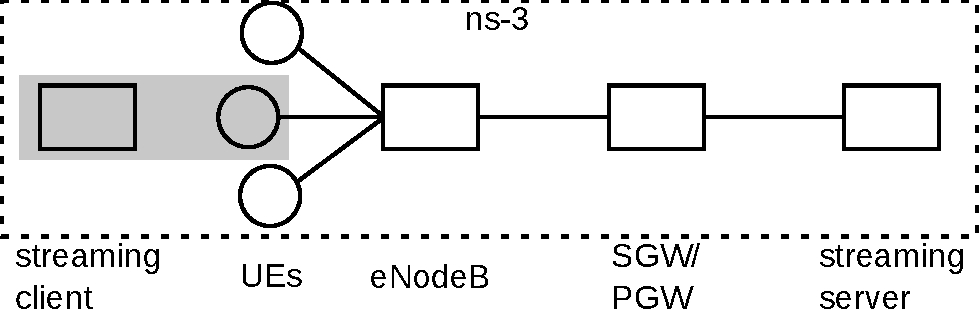
\includegraphics[width=0.6\textwidth]{images/streaming-simulation.pdf}
	\caption{\acrshort{LTE} reliable streaming simulation testbed.}
\label{c6:fig:streaming-simulation}
\end{figure}

The rest of the network model is kept as simple as possible as is visible in Figure~\ref{c6:fig:streaming-simulation}. LENA readily provides (incomplete) implementations for the \glspl{UE}, \gls{eNB}, and a combined \gls{SGW}/\gls{PGW} node. For the streaming simulation two things were added into this network: a streaming server and a streaming receiver and player.

For the streaming server a node from which the video segments are pulled was connected to the Internet-facing link of the \gls{PGW}. The storage server is kept as simple as possible. Upon receipt of a request for a specific segment over \gls{TCP} a dummy segment with the correct size is immediately sent to the client, reusing the open \gls{TCP} connection. %\todo{Segments typically have a size of ...?}
The \gls{TCP} congestion avoidance mechanism implemented by ns-3 is New Reno, which also might not be ideally suited to mobile environments. Especially when compared to newer congestion avoidance mechanisms that are optimized for a high \gls{BDP} like Linux's CUBIC.

In this setup \gls{TCP} will be directly used to transport the stream instead of for example the more commonly used application layer protocol \gls{HTTP}. This should make no difference on the streaming process in the long run apart from the absence of a slight protocol overhead (i.e., the \gls{HTTP} headers) at the beginning of the transmission and for each segment. Although some features coming with \acrshort{HTTP}/2 can not be easily tested in this way, especially the application layer multiplexing aspects. However, using \gls{TCP} directly simplifies the simulation and makes the results easier to interpret.

The client's playback buffering model is implemented as an application running on the \gls{UE}. The device also initiates the streaming and takes care of requesting each individual segment. For the purpose of this simulation the segments do not contain actual video data. Rather, the playback simulator just reads the list of frames and their size and synchronizes this information with the received amount of data to correctly calculate the buffer level.

During transmission, the existing \gls{LTE} framework sets up the lower layer protocols, which includes the radio stack and the \gls{gtp} core network bearer, accordingly. In the simplest model, only one \gls{eNB} and one \gls{UE} are present, to avoid interference with other devices. Additionally, a mobility model has to be selected for the \gls{UE} to be streamed to in order to conduct the experiments. The simplest case would be a stationary mobility model at a close distance to the transceiver, laying more emphasis on testing the influence of the overall network path rather than mobility factors. This should also give a measure of the upper limit of the achievable reliable streaming performance, all other mobility models will undoubtedly reduce the performance.

The scenario can now be easily extended to factor in multiple devices and an actual mobility model with handovers. The necessary capabilities to set this up are already present in ns-3's \gls{LTE} model. Apart from the described settings the \gls{LTE} nodes are otherwise left at their default configuration, which should yield an overall net bandwidth of \SI{80}{\mega\bit\per\second} in the \gls{LTE} radio cell.

\begin{figure}[htb]
	\centering
	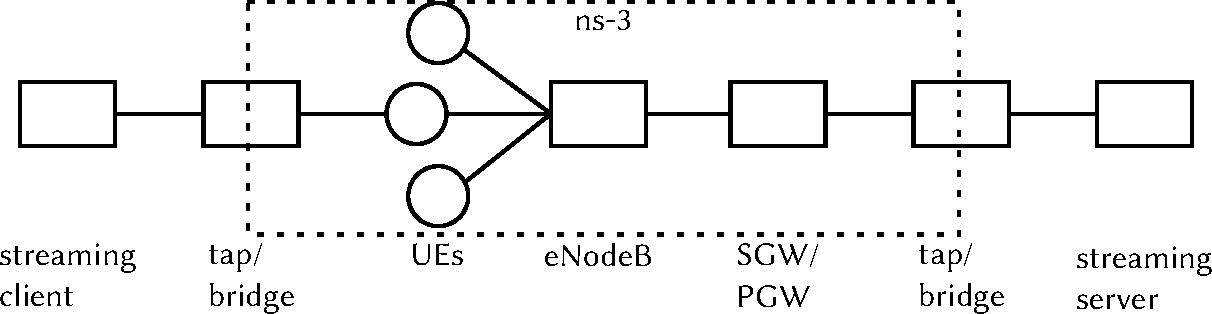
\includegraphics[width=1.0\textwidth]{images/streaming-hybrid.pdf}
	\caption{Future testbed iteration: hybrid of ns-3 \acrshort{LTE} simulation and actual or emulated streaming client and server bridged to it.}
\label{c6:fig:streaming-hybrid}
\end{figure}

Beyond its application as a pure simulation, a simulated ns-3 \gls{LTE} network could additionally be facilitated as a network emulator. Figure~\ref{c6:fig:streaming-hybrid} demonstrates such a setup. To be able to use it for a streaming emulation in the style of the measurements conducted in Section~\ref{c3:sec:measurements} a bridging device would need to be added on each side of the network, that interfaces with a real testbed network. The only task of the simulated part is then to alter the \gls{QoS} parameters of the link according to its model. This approach is ideally suited to quickly test existing and already implemented streaming solutions for use with a mobile network and saves the effort of reimplementing them as a simulation model.


%%
\subsubsection{Simulated Streaming Models}

Following the classifications and playback models from Sections~\ref{c3:sec:background} and \ref{c3:sec:model} the simulated model is a pull-based segmented video streaming system using \gls{TCP}. Two streaming models are suggested here, with the first suited for plain reliable streaming and the second modified to utilize the benefits of adaptive streaming. Other playback models could be easily implemented as well, but these to should closely resemble the usual approaches taken by real reliable streaming players as previously already observed.


%%
\paragraph{Four Threshold Segmented Streaming Strategy}

The first playback strategy is governed by four thresholds. They are, in the order of the buffer level, from lowest to highest, they represent:
%
\begin{enumerate}
	\item \textit{Playback stop}. Represents the lower limit of the buffer and the player will stop if the level goes below this threshold. It can be set to as low as \SI{0}{\second} but it defaults to \SI{0.5}{\second} for this model. When the limit is underrun, stalling will occur.

	\item \textit{Transmission start}. If the transmission is currently stopped due to reaching the buffer limit, restart it if it falls beyond this threshold. Naturally, at the start of the streaming process segments are already requested at a buffer level of zero. The default is set to \SI{2.5}{\second} of video in the buffer. The gap between this and the playback stop threshold should be large enough to avoid stalls because of transmission restarts occurring too late.

	\item \textit{Playback start}. This threshold takes effect after every stalling event and restarts the player if at least this amount is in the buffer. It is set to \SI{5}{\second} here.

	\item \textit{Transmission stop}. In some scenarios this last threshold might not be necessary as it only acts to prevent a buffer overrun and lost video data. But most mobile devices suffer from rather low memory constraints and therefore need to limit the video buffer. When this limit is reached, no new segments are requested until the buffer falls below the transmission start limit again. It is set to \SI{10}{\second} here and is a soft limit that can be exceeded by already requested segments that have yet to arrive. Therefore, it always should be set slightly below the buffer's actual hard limit.
\end{enumerate}


\begin{figure}[htb]
	\centering
	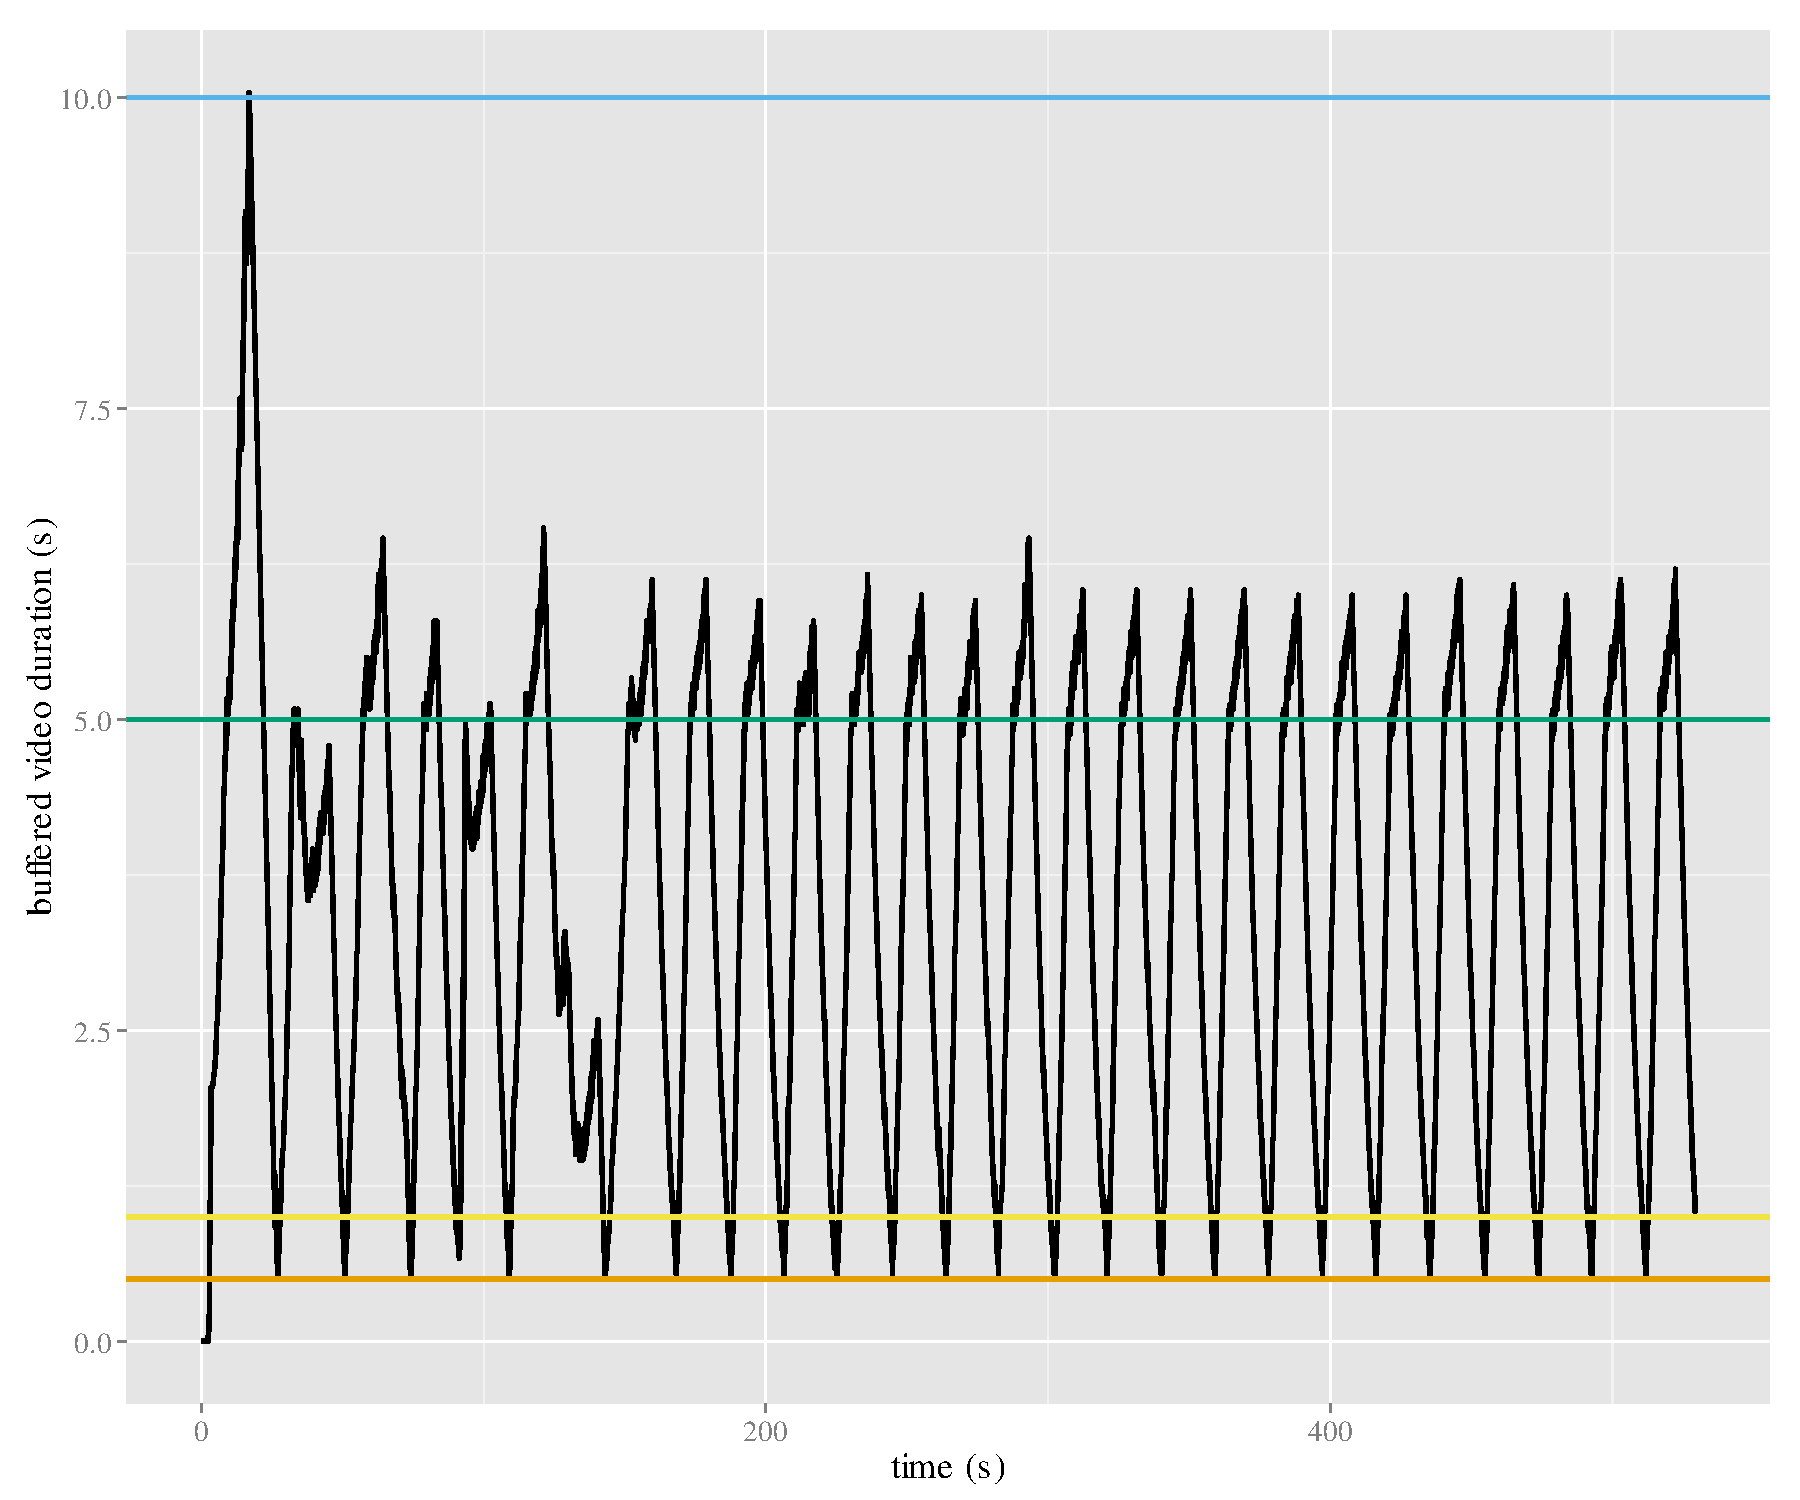
\includegraphics[width=0.9\textwidth]{images/R-ltesim-plotbuffer-time.pdf}
	\caption{Sample simulation run demonstrating the four threshold strategy.}
\label{c6:fig:ltesim-plotbuffer-time}
\end{figure}

To demonstrate the strategy an example scenario is displayed in Figure~\ref{c6:fig:ltesim-plotbuffer-time}. Depending on the relation of \gls{TCP} goodput to video bitrate a player with this strategy should always bounce between the transmission start and stop thresholds and never stop playing intermittently as in the example. The default threshold values given here may be far from ideal and need to be optimized in the long run. But this is often the same case in real streaming solutions with the players arbitrarily preconfigured to values that could make sense from the developer's point of view without scientific validation.


%%
\paragraph{Six Threshold Window Scaling Adaptive Streaming Strategy}

By adding two additional thresholds the strategy could also be extended to work for adaptive reliable streaming. As a further prerequisite, all video segments need to be available in a number of quality levels and therefore video bitrates and seamless switching between levels at the segment borders needs to be possible. The more quality levels are present the better adaptable the streaming client can be. It can already work with as low as two levels, but this coarse switching between a very low number of levels will also be more noticeable by the user and might disturb her \gls{QoE} more than a smooth decline in image quality.

The two new thresholds are values to trigger the switch to the next higher and lower segment quality level respectively. The reduce to lower quality threshold should be located between transmission start and playback stop, the increase to higher quality situated between playback start and transmission stop. To accommodate more than two levels these two thresholds can be triggered multiple times. If the buffer level is still rising after the segment quality has been raised the quality should be raised again at the next opportunity.

To better find a stable segment level candidate, the player should compute and keep track of the incline of the buffer level in the last time window. The steeper it gets the higher the chance for a quality level change should be. The same rule applies also to the lower quality threshold. Any adaptive streaming strategy should also avoid flapping back and forth between quality levels. This is usually conducted through some kind of hysteresis.

%While general quality changing support is present in the simulation model, this strategy is not fully implemented, but the basic four threshold strategy can be easily extended to match the adaptive strategy.


%%
\subsubsection{Scenario Evaluation}

To test the basic viability of the streaming simulation model (the validity \gls{LTE} model is taken as-is and covered by other research~\cite{Baldo:2013:OSM:2507924.2507940}) several test scenarios are defined and subsequently evaluated. Common to them is the configuration of the video streaming simulation module. In every case the simpler four threshold strategy is facilitated and tested with the three videos described in Table~\ref{c6:tbl:simulationvideos}, each representing a different quality profile. Only one simulation run was conducted for each parameter setting as there are no known random factors involved that would merit running with different random seeds.

\begin{table}[htb]
\caption{Parameters of the video used in the streaming simulation scenarios.}
\label{c6:tbl:simulationvideos}
	\centering
	\begin{tabu}{X[1.5,l]X[r]X[r,1.2]X[r]}
		\toprule
		\textbf{Parameter} & \textbf{Low Quality} & \textbf{Standard Quality} & \textbf{High Quality} \\
		\midrule
		Video duration  & \SI{318}{\second} & \SI{602}{\second} & \SI{596}{\second} \\
		Size & \SI{19.2}{\mebi\byte} & \SI{258}{\mebi\byte} & \SI{853}{\mebi\byte}\\
		Frame rate & \SI{29.97}{\per\second} & \SI{29.97}{\per\second} & \SI{24}{\per\second}\\
		Average video bitrate & \SI{504}{\kilo\bit\per\second} & \SI{3596}{\kilo\bit\per\second} & \SI{12}{\mega\bit\per\second} \\
		Codec & H.263 & MPEG-4 & MPEG-4 \\
		\bottomrule
	\end{tabu}
\end{table}


%%
\paragraph{Congested Server Link}

This first series of evaluations exclusively looks at the \gls{QoS} of the streaming server's link and leaves the \gls{LTE} configuration unaltered. The radio subsystem is configured to have a stationary \gls{UE} in close vicinity of the single \gls{eNB}. It should therefore reach the maximum attainable performance of radio link as it will be undisturbed by other users and fading effects. Therefore, it also represents the best case scenario for mobile streaming. If the streaming strategies and the associated video files reveal issues under these conditions they will surely also fail in an environment with a more degraded radio link.

The \gls{QoS} variables altered here are the link's bandwidth and delay. Loss will remain unchanged and at zero, as it will also result in just another source of delay for the reliable streaming process due to retransmission. Similar to the evaluations with the measurement framework of Section~\ref{c3:sec:measurements} the performance will be measured on the basis of the player's stalling characteristics, i.e., the total duration and the number of stalling phases. With this, more complex \gls{QoE} metrics can then be calculated.

\begin{figure}[htb]
	\centering
	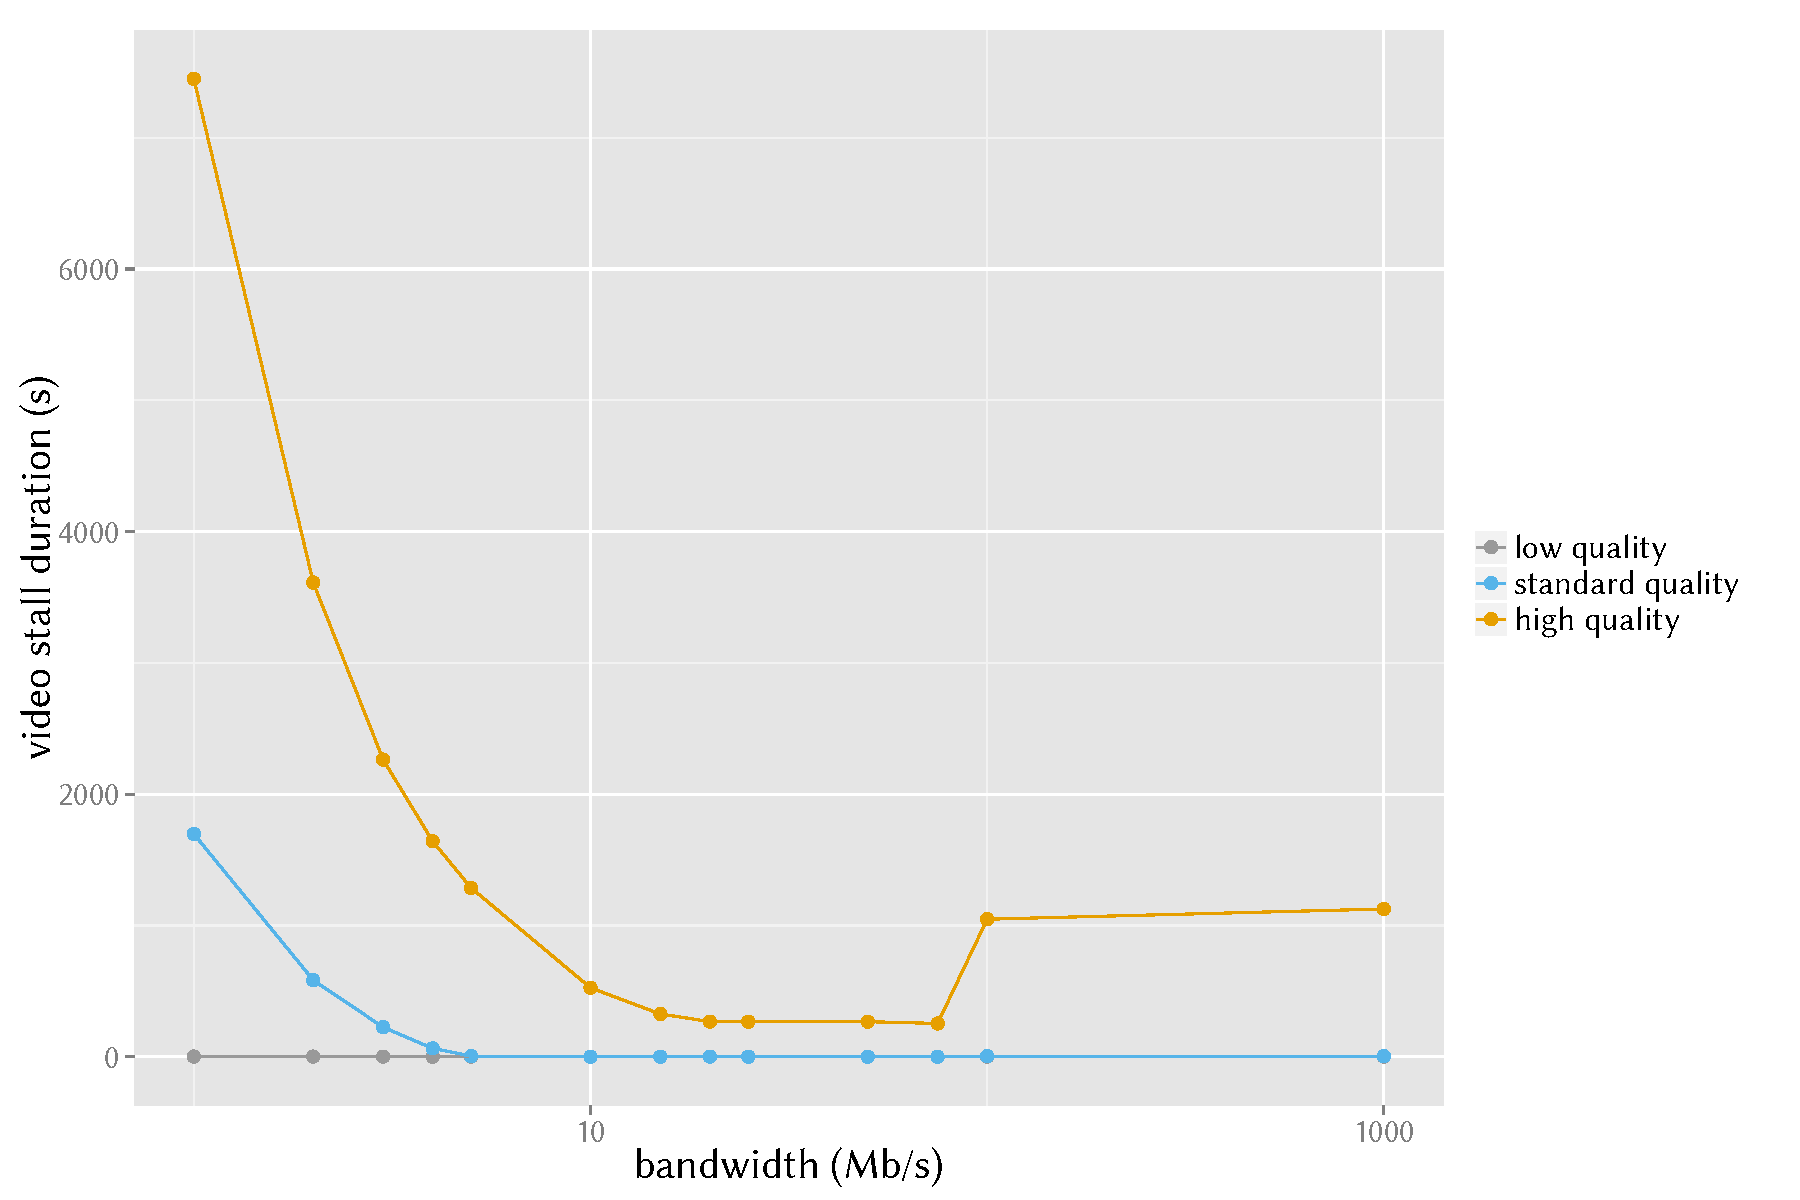
\includegraphics[width=0.9\textwidth]{images/R-ltesim-bwseries-stallduration.pdf}
	\caption{Relative stalling duration of the simulated reliable streaming player under limited Internet bandwidth.}
\label{c6:fig:ltesim-bwseries-stallduration}
\end{figure}

\begin{figure}[htb]
	\centering
	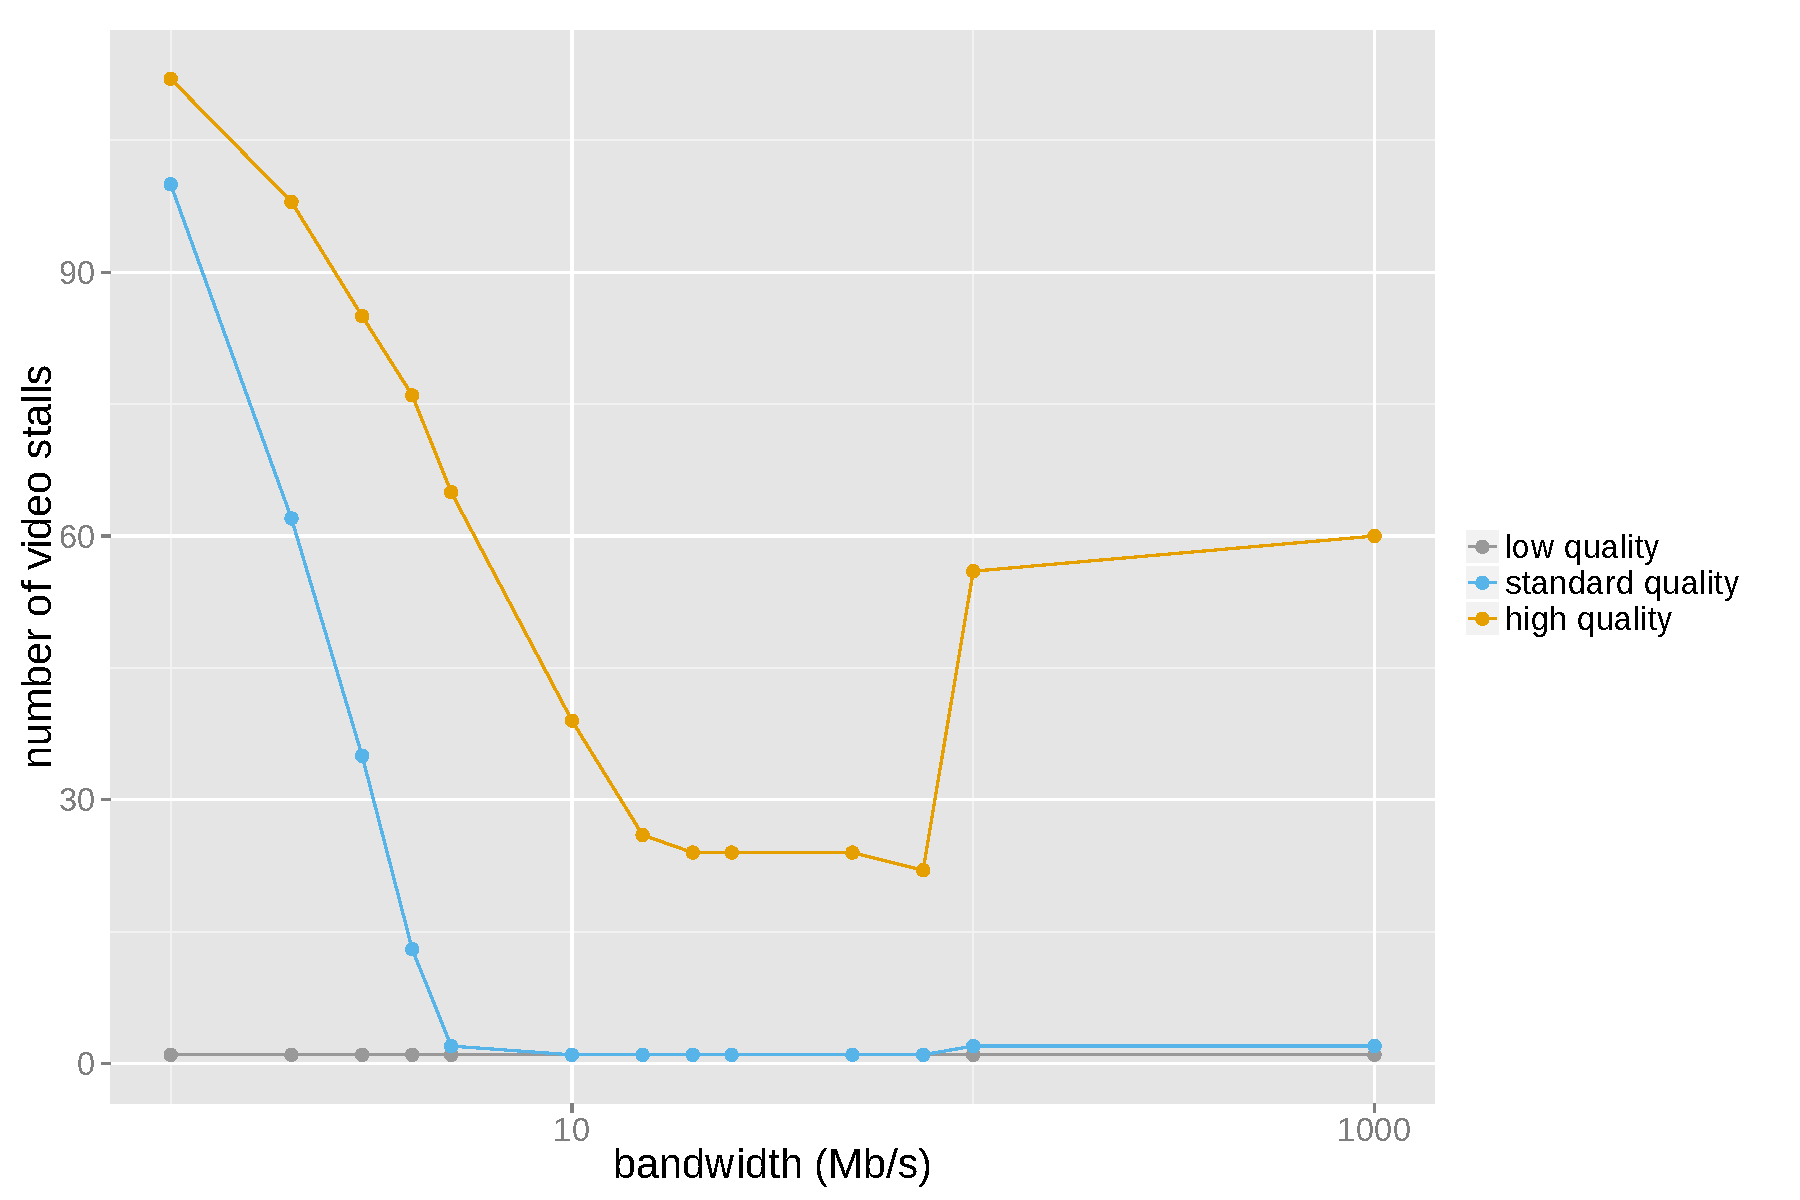
\includegraphics[width=0.9\textwidth]{images/R-ltesim-bwseries-numstalls.pdf}
	\caption{Number of stalling events of the simulated reliable streaming player under limited Internet bandwidth.}
\label{c6:fig:ltesim-bwseries-numstalls}
\end{figure}

The first series solely alters the bandwidth of the streaming server's link up to a maximum of \SI{1000}{\mega\bit\per\second}. The results are depicted in the Figures~\ref{c6:fig:ltesim-bwseries-stallduration} and \ref{c6:fig:ltesim-bwseries-numstalls}.

As soon as the link's bandwidth exceeds the video's bit rate, the number and duration of stalls are reduced. Stall events and duration in both the low and standard quality videos drop to zero. Only the high quality video does not show the same results. As its bit rate of \SI{12}{\mega\bit\per\second} should be perfectly manageable for the radio link some other explanation is required. A possible hypothesis are issues with the approach to requesting subsequent segments. As these need to be requested in a timely manner while other segments are still being transmitted, they could be requested to late and do not saturate the link anymore. 

However, this effect is somewhat contrary to the additional effect observed at link speeds of \SI{100}{\mega\bit\per\second} and above, where the stalling phases suddenly see an unexpected increase. As this happens exactly when the transmission speed exceeds the radio links capacity of about \SI{80}{\mega\bit\per\second} it might be an indication of the negative interaction of \gls{LTE}'s loss and congestion concealment with \gls{TCP}'s congestion avoidance mechanisms, related to the previously discussed bufferbloat issues. \gls{TCP} can not properly detect the bottleneck capacity in a timely manner as \gls{LTE} attempts to buffer and retransmit any packet exceeding the radio capacity below the user \gls{IP} layer. Through this issue, the effective goodput seems to get reduced to about \SI{5}{\mega\bit\per\second}, which is not enough for the high quality video to stream without interruption.

\begin{figure}[htb]
	\centering
	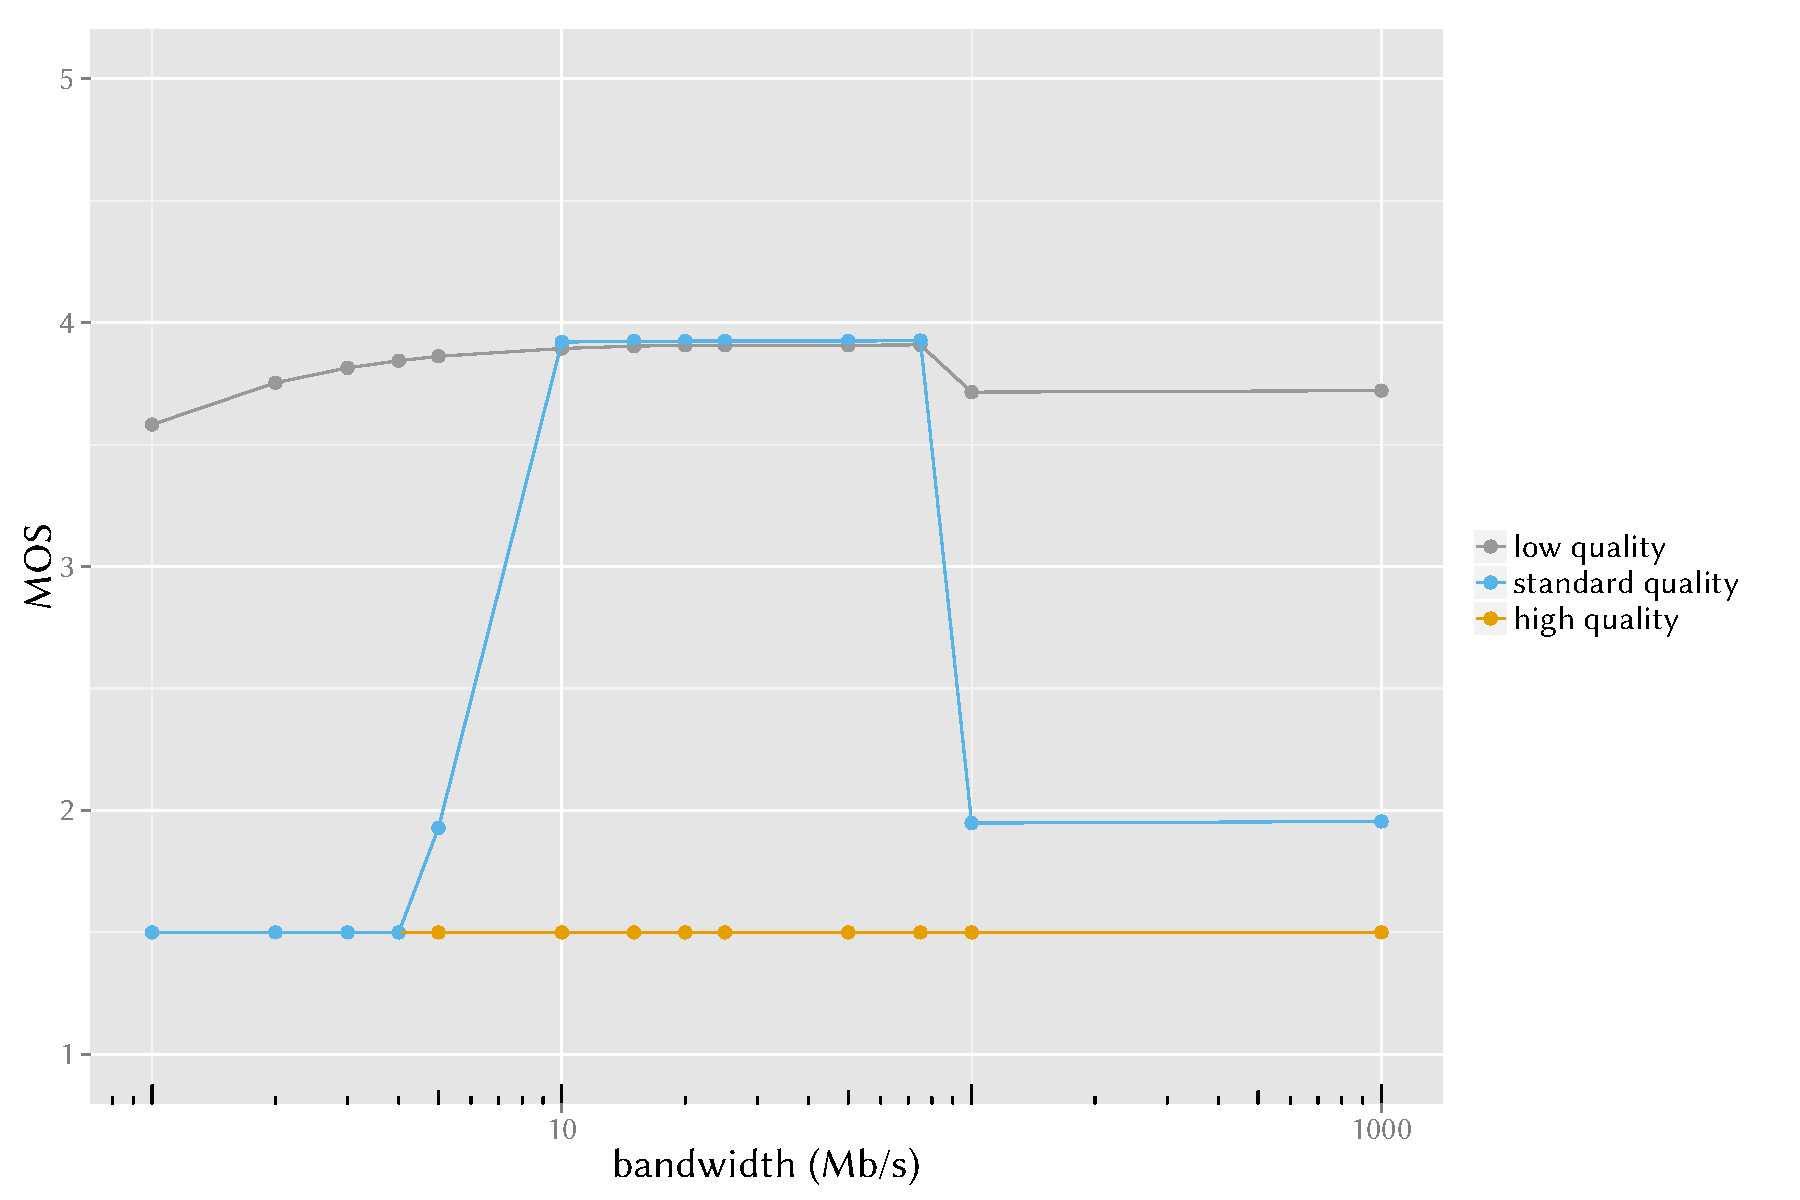
\includegraphics[width=0.9\textwidth]{images/R-ltesim-bwseries-qoe.pdf}
	\caption{Computed \acrshort{QoE} of the reliable streaming strategy with limited bandwidth.}
\label{c6:fig:ltesim-bwseries-qoe}
\end{figure}

Once again utilizing Equation~\ref{c3:eqn:hossfeld-stalling-model} as a validated \gls{QoE} metric and applying it to the results of the bandwidth series, it is evident that the perceived quality really suffers in this scenario. The \gls{MOS} of the high quality video never exceeds the equations base value of $1.5$ and is effectively unwatchable according to the metric. The other two video profiles manage to achieve a good quality when sufficient bandwidth is present, with the issues above \SI{80}{\mega\bit\per\second} in mind.


%\todo{check pcaps for >=100mbit experiments; could also be related to issues of the actual lte simulation network but implementation can not fully responsible for this?}

\begin{figure}[htb]
	\centering
	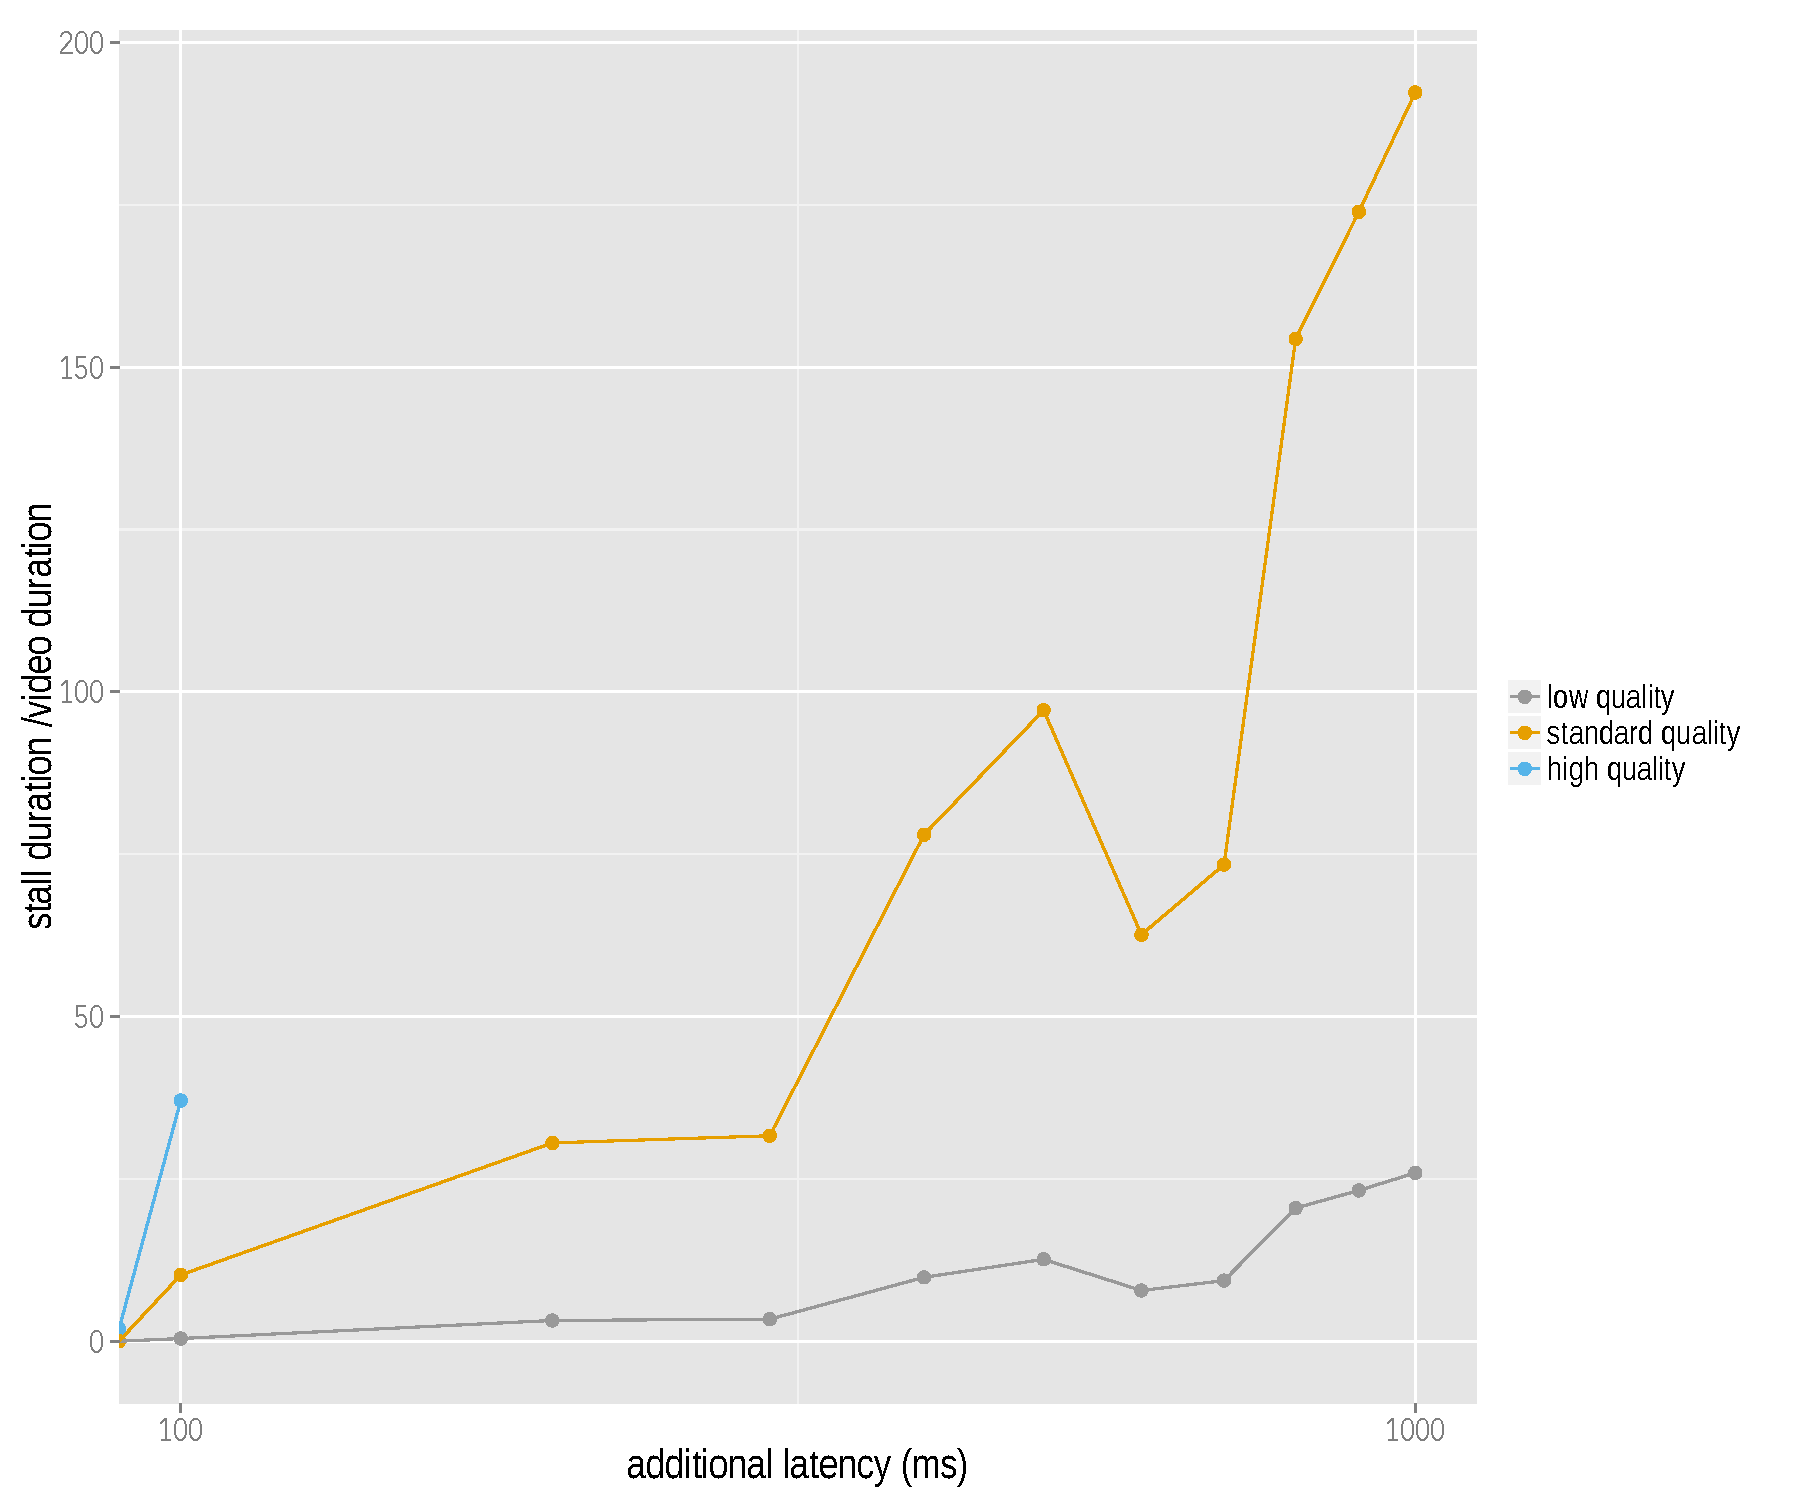
\includegraphics[width=0.9\textwidth]{images/R-ltesim-latencyseries-stallduration.pdf}
	\caption{Relative stalling duration of the simulated reliable streaming player under increased Internet latency.}
\label{c6:fig:ltesim-latencyseries-stallduration}
\end{figure}

\begin{figure}[htb]
	\centering
	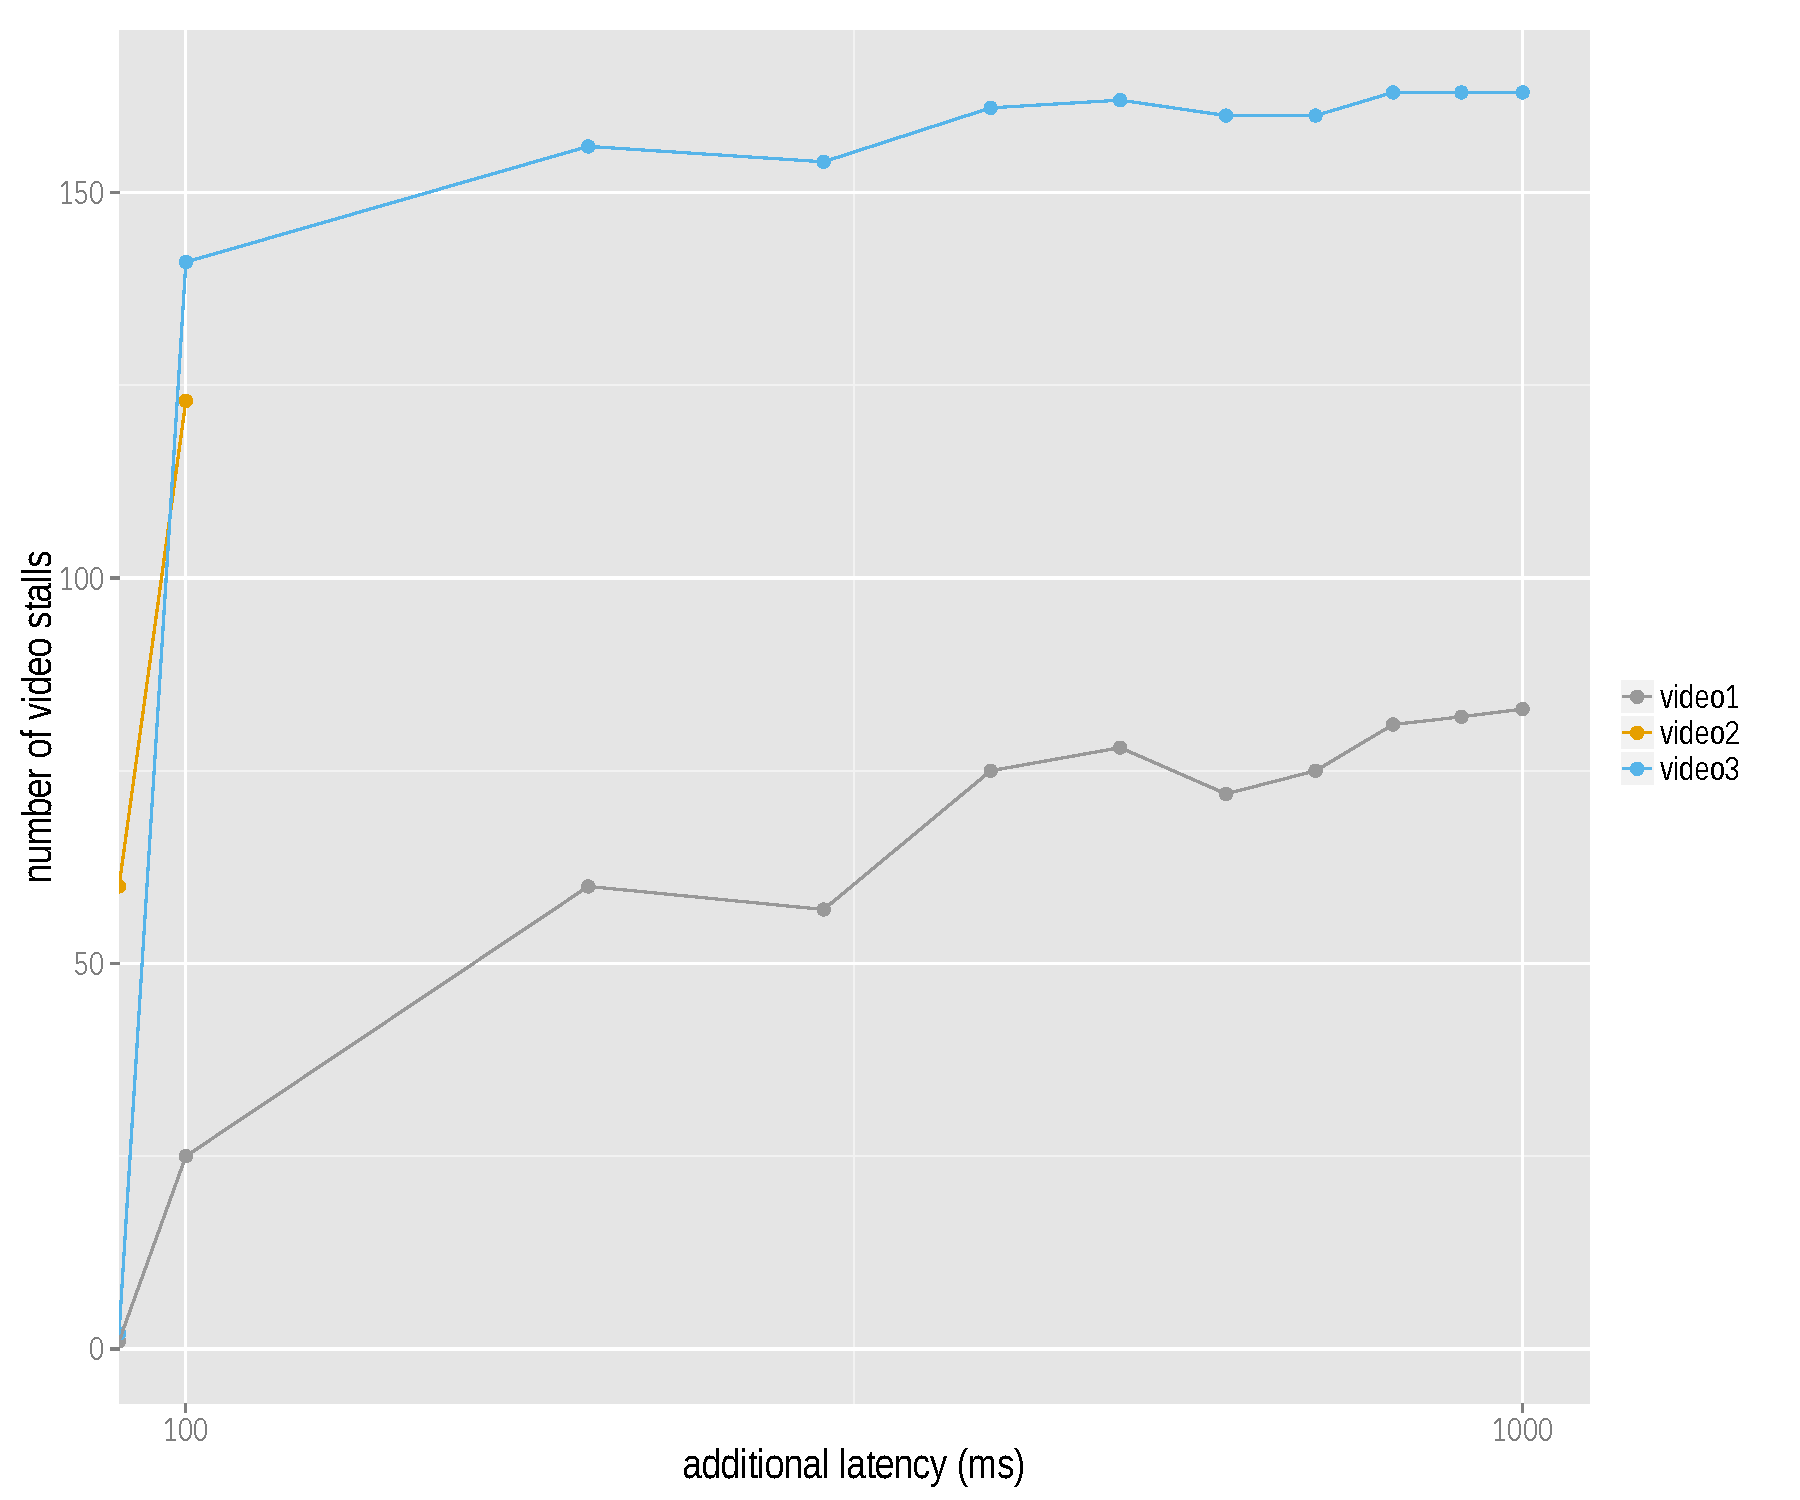
\includegraphics[width=0.9\textwidth]{images/R-ltesim-latencyseries-numstalls.pdf}
	\caption{Number of stalling events of the simulated reliable streaming player under increased Internet latency.}
\label{c6:fig:ltesim-latencyseries-numstalls}
\end{figure}

In a second series of simulation runs the latency of the streaming server's link was increased incrementally up to an additional latency of \SI{1000}{\milli\second}. The values were set deterministically with no probability distribution. Figures~\ref{c6:fig:ltesim-latencyseries-stallduration} and \ref{c6:fig:ltesim-latencyseries-numstalls} again show the results in terms of the relative duration and number of stalling phases. The playback simulation seems to be excessively sensitive to latency increases. Even a small \SI{100}{\milli\second} increase makes the high and standard quality videos completely unwatchable as the stalling duration is more than ten times longer than the actual video. With latencies beyond \SI{100}{\milli\second} the high quality video could not be successfully streamed anymore. The computed \gls{QoE} of this scenario is not displayed as it essentially never deviates from the base \gls{MOS} of $1.5$, verifying the detrimental impact of the latency.

This behavior can partially be attributed to the simplistic segment request strategy used in this experiment. New segment are only requested when the previous one has fully arrived. As this takes a full round trip, the latency has a significant influence on the arrival time of subsequent segments. To avoid this kind of stop-and-wait behavior in the segment request process, new segments need to be requested sufficiently in advance while the previous segment is still being transmitted, so that the full bandwidth is always utilized. With these improvements to the retrieval strategy this specific issue can be eliminated. But this just shows one of the many pitfalls and influences of various layers. A simple implementation detail may have large implications on the streaming quality the user experience.


%%
\paragraph{Device Mobility}
\label{c6:sec:mobilitystreamingsim}

\begin{figure}[htb]
	\centering
	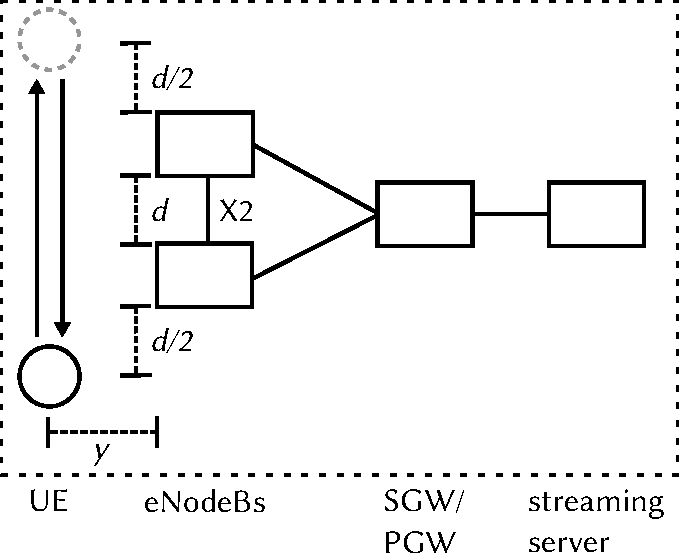
\includegraphics[width=0.5\textwidth]{images/streaming-simulation-mobility.pdf}
	\caption{Simulated handover mobility scenario using waypoints.}
\label{c6:fig:streaming-simulation-mobility}
\end{figure}

Besides altering the server link, the effects of the simulated \gls{LTE} network can also be investigated through various other means. In the following scenario mobility will be under scrutiny. For this, a second \gls{eNB} will be added to the network. Both are connected through the X2 interface, which will be used for the \gls{eNB}-anchored mobility provided by ns-3's \gls{LTE} model.\@ Instead of having a constant position relative to the \gls{eNB}, the \gls{UE} will now move back and forth between two waypoints on a two-dimensional plane in parallel to the two base stations which are placed at a distance of $d$ between each other. A handover is triggered each time the device leaves the range of one station and enters the other. Furthermore, the horizontal distance on the 2D-plane between the device and the \glspl{eNB} is controlled by a second parameter $y$. Figure~\ref{c6:fig:streaming-simulation-mobility} depicts this scenario and the positioning of the waypoints.

\begin{figure}[htb]
	\centering
	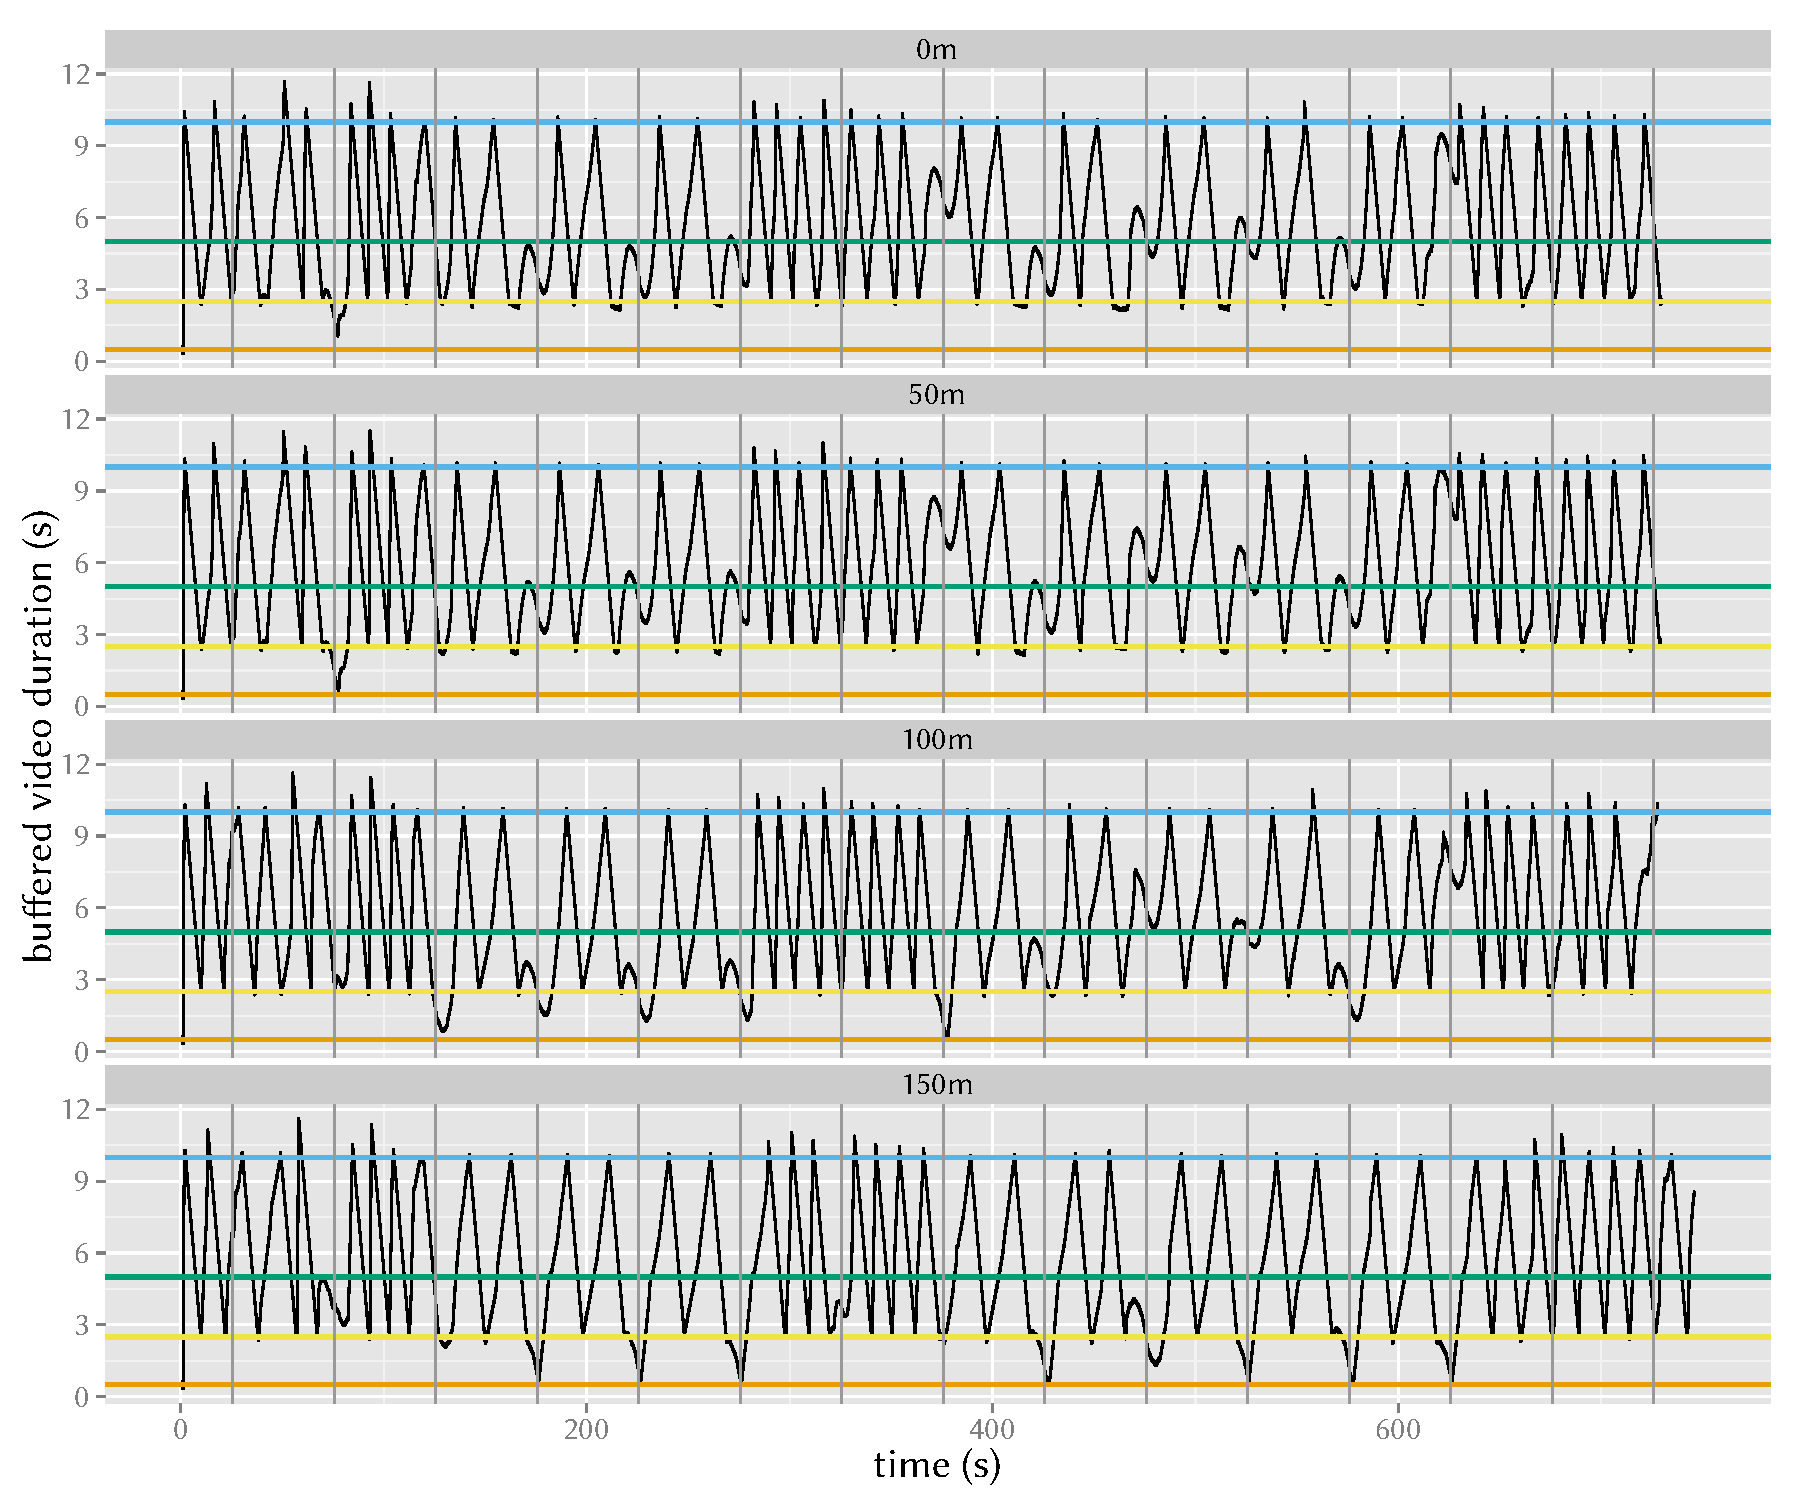
\includegraphics[width=0.9\textwidth]{images/R-ltesim-plotbuffer-mobility-facets.pdf}
	\caption{Playback buffer time series of the simulated mobility experiments with increasing distance between device and \acrshortpl{eNB}.}
\label{c6:fig:ltesim-mobility-plotbuffer-facets}
\end{figure}

For the purpose of this experiment, the two \glspl{eNB} were placed at a vertical distance of $d=\SI{500}{\meter}$ while the horizontal distance to the device was varied between $y=\SI{0}{\meter}$ and $y=\SI{150}{\meter}$. The device is moving at a constant velocity of \SI{20}{\meter\per\second}. During the movement the standard quality video was streamed to the device and its playback simulated. The results in terms of the buffer fill level are displayed in Figure~\ref{c6:fig:ltesim-mobility-plotbuffer-facets}. The color-coded horizontal lines once again demark the same thresholds from the previously described four threshold segmented streaming strategy.

The handover events between the two \gls{eNB} are denoted by the gray vertical lines and occur in regular intervals. The actual control transfer usually last for only about \SI{40}{\milli\second}. But looking at the figures it is immediately evident that the video buffer, and therefore the throughput of the video segments, already suffers seconds before this handover event when the edge of the radio range of the currently active \gls{eNB} is reached. The playback stop threshold is undercut several times right at the handover mark resulting in a playback stalling phase.

It seems, that the throughput at the radio edge drops below the video's average bitrate of \SI{3596}{\kilo\bit\per\second}. Therefore, the buffer cannot be maintained for this quality level. If the buffer was at a critically low level beforehand, it will run empty and lead to stalling due to the mobility. Additionally, there seems to be a dependency between the stalling probability and the distance between device and base station. A farther distance decreases the achievable throughput leading to an increased chance of the buffer running empty.

Mobile streaming playback strategies can attempt to counteract mobility-related issues in a number of ways. A simple approach would be to adjust the threshold levels to allow for a much larger buffer while also restarting transmissions earlier. But this comes at the price of an increased memory resource usage on the device, which might not possible in every scenario. Second, the strategy can be exchanged for an adaptive one, for example the described six threshold window scaling strategy with appropriately chosen threshold values. Here, the stalls are exchanged for phases of lower quality video, which can be acceptable under circumstances. 

Finally, both non-adaptive and adaptive strategies can be improved by employing the cross-layer model described in Section~\ref{c5:sec:crosslayerhinting}. By utilizing information from the radio network layers, handover events can be detected sufficiently in advance and an appropriate reaction chosen by the playback strategy. For example by temporarily increasing the maximum buffer threshold and requesting segments more rapidly or by quickly dropping to a lower quality level and filling the buffer up.

%%
\paragraph{Further Scenarios}

Apart from the experiments conducted here, some others scenarios listed here are also worth investigating but out of scope for this work.

If one plans to implement a reliable streaming solution, the simulation can be utilized to test any kind of playback strategy and transmission mechanics and attune it to mobile networks. Besides developing entirely new playback strategies, the default thresholds of the four and six threshold strategies should also be optimized through the iterative simulation of value combinations.

The opposite approach would also be possible for mobile network operators: Map the operator's mobile network infrastructure onto the simulation and test the performance of existing streaming strategies with it. If any issues or performance bottlenecks are discovered, the operator can make adjustments to the infrastructure and implement these changes afterwards outside of the simulation.

It would also be worthwhile to see the impact of the cross-layer model described in Section~\ref{c5:sec:crosslayerhinting} as they are specifically intended to reduce the influence this kind of mobile network architecture has on user applications. An implementation of cross-layer hinting would be relatively simple here, as the layer isolation boundaries are much easier to circumvent in a network simulator and information on, e.g., handover events is readily available.

As mentioned earlier, ns-3's \gls{LTE} framework does only implemented a limited subset of the \gls{3GPP} specifications, mainly related to the user plane and the radio link stack. Almost no control plane procedures are implemented. This may have only a negligible impact as soon as a connection is established and remains stable and only a very small number of users are connected to the system. But this is not the norm for an actual mobile network in operation with its mobility features and high churn, both in terms of data flows as well as mobile users, generating a large amount of signaling traffic as was discussed before in Section~\ref{c4:sec:3gpparchitecture}. To best mimic the dataset evaluations related to \gls{PDP} context and \gls{gtp} tunnel life cycle management conducted in Section~\ref{c4:sec:evaluations}, the simulator would need to at least be able to reproduce these tunnel management and the related \gls{RRC} \gls{PDP} context procedures happening on the user traffic path. Therefore, it is worth to reconduct the above experiments as soon as the framework has made any progress in this direction.




% \url{http://www.valid8.com/UMTS_Core_Network_Simulator.html} Not publicly available and commercial
% also seems to focus on the circuit switched domain


% Only commercial: UMTS model in OPNET (which was renamed to Riverbed Modeler)\footnote{\url{http://www.riverbed.com/products/performance-management-control/network-performance-management/network-simulation.html}} 
% again radio and user plane focused

%\url{http://www.nsnam.org/docs/release/3.20/doxygen/group__lte.html}
%\url{http://www.nsnam.org/docs/release/3.20/models/html/lte.html}

%Reasoning why ns-3/LENA will be used here.
%but combined with ns-3 offers almost complete representation of a vanilla network and transport level network stack


%performance: eNB has 25 resource block each up/down; suggests 5Mhz BW
%https://groups.google.com/forum/#!searchin/ns-3-users/lte/ns-3-users/dwMjWwJBdBw/wfWCcRctN4EJ



% LQ
% MP4 container
% 352x288
% AAC audio, 11KHz
% \SI{24.0}{\kilo\bit\per\second} audio bitrate)
% \SI{531.0}{\kilo\bit\per\second} overall bitrate
% SD
% DivX container
% 720x400
% MP3 audio, 44.1Khz
% \SI{128}{\kilo\bit\per\second} audio bitrate
% \SI{3735}{\kilo\bit\per\second} overall bitrate
% HQ
% AVI container
% 1920x1080
% AC-3 audio, 48Khz
% \SI{448}{\kilo\bit\per\second} audio bitrate
% \SI{12.5}{\mega\bit\per\second} overall bitrate
%%%%%%%%%%%%%%%%%%%%%%%%%%%%%%%%%%%%%%%%%%%%%%%%%%%%%%%%%%%%%%%%%%%%%%%%%%%%%%%%


\section{Summary}

It is safe to assume that reliable video streaming in mobile networks can be evaluated in a large number of ways. Besides the previously taken road of passively recorded network-scale traces, two other approaches are most valuable in investigating reliable streaming, active measurements and simulations. Both bring along their own set of benefits and drawbacks. 

Active measurements are better suited to test the wide range of influence factors present in actual networks and device protocol stacks. These can usually not be properly represented in a simulation. In order to increase the viability for mobile measurements, Sensorium was introduced, making it easier to record the precise state the mobile device currently is experiencing by giving access to all kinds of sensors.

If the goal is rather to investigate the theoretical overarching concepts of certain playback strategies or to scale up the test environment, one can utilize the simulative approach in the form of the \gls{LTE} mobile streaming simulation framework. Initial measurements using this framework already suggest a high influence of the network \gls{QoS} on the experienced streaming quality. A higher stalling probability caused by handovers during mobility was also uncovered.


%\section{Mobile Streaming and Measurement Summary}
%Cover both this and the previous Chapter?
%\todo{chapter summary required or fold it into thesis summary?}



%\url{http://www.wisebed.eu/}
%M-Lab \url{http://www.measurementlab.net/}

%Lessons Learned from the NetSense Smartphone Study 
%provided smartphones, subsidized by sprint
%just specific study, not a testbed

%OsmocomBB project \cite{osmocombbwww}


%An evaluation of dynamic adaptive streaming over \gls{HTTP} in vehicular environments \cite{Muller:2012:EDA:2151677.2151686}